% 参考サイト: http://www.is.nagoya-u.ac.jp/dep-ss/phil/kukita/others/How_to_use_TeX.pdf










\documentclass[titlepage]{jsarticle}




\usepackage[dvipdfmx]{graphicx} % 図の挿入
\usepackage[dvipdfmx]{color} % これがないと文字に色をつけたときに画像が真っ白になる
\usepackage{caption}
\usepackage{ascmac}  % 枠付き文章
\usepackage{amsmath} % 数式
\usepackage{comment} % 複数行コメント
% \usepackage{algorithmic}
\usepackage{algorithm}
\usepackage{algpseudocode}
% 定理
\usepackage{amsthm}
\newtheorem{thm}{定理}
\newtheorem{definition}[thm]{定義}
\newtheorem{example}[thm]{例}
% プログラムのソースコード
\usepackage{listings} % ソースコードを書けるようにする
\usepackage{jvlisting} % 日本語が文字化けしないようにする
\usepackage{jlisting}  % pythonにおいて日本語の位置が変わらないようにする
\lstset{ %↓ここはソースコードの書式設定
  basicstyle={\ttfamily},
  identifierstyle={\normalsize},
  commentstyle={\smallitshape},
  keywordstyle={\small\bfseries},
  ndkeywordstyle={\small},
  stringstyle={\small\ttfamily},
  frame={tb},
  breaklines=true,
  columns=[l]{fullflexible},
  numbers=left,
  xrightmargin=0zw,
  xleftmargin=3zw,
  numberstyle={\scriptsize},
  stepnumber=1,
  numbersep=1zw,
  lineskip=-0.5ex
}
\renewcommand{\lstlistingname}{ソースコード}


\newif\ifdraft
\drafttrue
\draftfalse

\usepackage{color}
\ifdraft
\newcommand{\todo}[1]{{\bf \color{red}{[{#1}]}}}
\else
\newcommand{\todo}[1]{}
\fi


% タイトル
\title{MiniSatと遺伝アルゴリズムを組み合わせた短い証明の作成}
\author{和田 翔太}
\date{\today}










% 本文
\begin{document}





\maketitle





\begin{abstract}
	本論文では、与えられた命題論理式が充足不能であることの短い証明を作る方法を与える。

	本研究の背景にはSATソルバの高速化という課題がある。充足可能性問題を解くSATソルバは広く利用されているため、その高速化は重要な課題である。

	短い証明を作ることは、この問いに関する間接的な答えを与える。
	SATソルバは充足不能な命題に対して充足不能性の証明を与えるため、証明の長さの下限は理想的なSATソルバの実行時間の下限となる。 

	本論文では既存のSATソルバの中でも比較的改造が簡単な MiniSat に対して改造を行い、特定のタイミングで選択する変数を変更したり、変数の重みを変更したりするなど、変数選択へ介入を行った。
	そして、遺伝アルゴリズムを使用し、短い証明が作れるような重み変更のタイミングとその重みの解を探索することで様々な問題に対して短い証明を作成した。

	実験の結果として、次のような観察を得た。
	特定のタイミングで変数選択を変更してもあまり短い証明が得られないこと、遺伝アルゴリズムを MiniSat に使用することで使用する前の MiniSat よりも短い証明を作れることがわかった。
	しかし、問題によっては現在の高速なSATソルバである Kissat が作る証明よりも短い証明は作れていない場合もあり、短い証明ができても Kissat が作る証明の100倍短くなるような大幅に短い証明はできていない。
\end{abstract}





\tableofcontents
\newpage
















\input{introduction.tex}







\section{準備}





\subsection{SAT}



SATとは命題論理式の充足可能性を判定する問題でSatisfiability Problemの頭3文字を取ってSATと呼ばれる。
これは与えられた命題論理式を真にするような各変数への割り当てが存在するかどうか(充足可能かどうか)判定するという問題である。
命題論理式を真にするような各変数への割り当てが存在する場合は充足可能(SAT), 各変数にどのような割り当てをしても全体が真にならない場合は充足不能(UNSAT)となる。
通常SATである場合はその解(各変数への割り当て)を出力する。

\begin{definition}[命題変数]
	真を表す$\top$または偽を表す$\bot$を値にとる変数
	\[
	x_1, x_2, \ldots
	\]
	を命題変数と呼ぶ。
\end{definition}
命題変数それ1つでも論理式となる。
\begin{example}
	命題変数$x_1$は1変数からなる論理式となる。
\end{example}
命題論理式はこれらの命題変数を組み合わせることで表現される。

次に命題変数$x_1, x_2, \ldots $に対して操作を表す記号$\lor, \land, \neg$を導入する。
これらの記号は論理演算子と呼ばれ、それぞれ論理和、論理積、否定と呼ばれる。
\begin{comment}
命題変数$x_i$と$x_j$の論理和を$x_i \lor x_j$で表す。$x_i$と$x_j$がどちらも偽である場合に偽になり、それ以外の場合は真となる。
また、命題変数$x_i$と$x_j$の論理積$x_i \land x_j$で表す。$x_i$と$x_j$がどちらも真である場合に真になり、それ以外の場合は偽となる。
\[
	x_i \lor x_j = 
	\begin{cases}
		\bot & (x_i=x_j=\bot{の場合}) \\
		\top & ({それ以外の場合}) \\
	\end{cases}
	, 
	x_i \land x_j = 
	\begin{cases}
		\top & (x_i=x_j=\top{の場合}) \\
		\bot & ({それ以外の場合}) \\
	\end{cases}
\]

命題変数$x$に対してその否定を$\neg x_i$で表す。$x_i$が真である場合に$\neg x_i$は偽になり、$x_i$が偽である場合に$\neg x_i$は真となる。
\[
	\neg x_i =
	\begin{cases}
		\bot & (x_i=\top{の場合}) \\
		\top & (x_i=\bot{の場合}) \\
	\end{cases}
\]
\end{comment}

以下、$x_i$と$x_j$を命題変数とする。

\begin{definition}[論理和]
	$x_i \lor x_j$を$x_i$と$x_j$の論理和と呼ぶ。
	$x_i$と$x_j$がどちらも偽である場合に偽になり、それ以外の場合は真となる。
	\[
		x_i \lor x_j = 
		\begin{cases}
			\bot & (x_i=x_j=\bot{の場合}) \\
			\top & ({それ以外の場合}) \\
		\end{cases}
	\]
\end{definition}

\begin{definition}[論理積]
	$x_i \land x_j$を$x_i$と$x_j$の論理積と呼ぶ。
	$x_i$と$x_j$がどちらも真である場合に真になり、それ以外の場合は偽となる。
	\[
		x_i \land x_j = 
		\begin{cases}
			\top & (x_i=x_j=\top{の場合}) \\
			\bot & ({それ以外の場合}) \\
		\end{cases}
	\]
\end{definition}

\begin{definition}[否定]
	$\neg x_i$を$x_i$の否定と呼ぶ。
	$x_i$が真である場合に$\neg x_i$は偽になり、$x_i$が偽である場合に$\neg x_i$は真となる。
	\[
		\neg x_i =
		\begin{cases}
			\bot & (x_i=\top{の場合}) \\
			\top & (x_i=\bot{の場合}) \\
		\end{cases}
	\]
\end{definition}

上記の論理演算子を命題変数と組み合わせたものは論理式となる。
\begin{example}
	$\neg x_i$は1変数からなる論理式になる
\end{example}
\begin{example}
	$x_i \lor x_j, x_i \land x_j$はそれぞれ2変数からなる論理式になる。
\end{example}

論理式$X_i, X_j$に対しても命題変数と同様に論理式の論理和$X_i \lor X_j$, 論理積$X_i \land X_j$, 否定$\neg X_i$を定義することができる。

上記の3つの論理演算子とは他の演算子として排他的論理和$\oplus$, 含意$\to$, 同値$\leftrightarrow$があるが、
今回のSATの問題を表現する際に用いないので省略する。
実際には排他的論理和$\oplus$, 含意$\to$, 同値$\leftrightarrow$は全て論理和$\lor$, 論理積$\land$, 否定$\neg$を用いて表現できるため、
6つ論理演算子で表現できる論理式は全て論理和$\lor$, 論理積$\land$, 否定$\neg$を用いて表現できる。

SATの問題は通常、連言標準形(conjunctive normal form; CNF)と呼ばれる特定の形式の論理式で表現される。

\begin{definition}
	命題変数$x_i$または命題変数の否定$\neg x_i$をリテラルと呼ぶ。
\end{definition}

\begin{definition}
リテラル$l_1, l_2, \ldots, l_n$に対してそれらを論理和$\lor$でつないだ論理式
\[
	l_1 \lor l_2 \lor \cdots \lor l_n
\]
を節と呼ぶ。
\end{definition}

SATの問題(CNF式)はこの節を論理積でつないだ論理式で表現される。

\begin{definition}
	節$C_1, C_2, \ldots, C_m$に対してそれらを論理積$\land$で繋いだ論理式
	\[
		C_1 \land C_2 \land \cdots \land C_m = (l_{11} \lor l_{12} \lor \cdots \lor l_{1n_1}) \land (l_{21} \lor l_{22} \lor \cdots \lor l_{2n_2}) \land \cdots \land (l_{m1} \lor l_{m2} \lor \cdots \lor l_{mn_m})
	\]
	をCNF式と呼ぶ
\end{definition}

\begin{example}
	論理式$(x_1 \lor x_2) \land (\neg x_3 \lor x_4)$はCNF式である
\end{example}

\begin{example}
	論理式$(x_1 \land x_2) \lor (\neg x_3 \lor x_4)$はCNF式ではない
\end{example}

また節をリテラルの集合で表し、CNF式を節の集合で表すことがある。
先ほどの例のCNF式$(x_1 \lor x_2) \land (\neg x_3 \lor x_4)$は$\{\{x_1, x_2\}, \{\neg x_3, x_4\}\}$といった集合で表現される。

最後に充足可能、充足不能について定義する。

まず割当を定義する。
\begin{definition}[割当]
命題変数についてその割当(未割当も含める)を写像
	\[
		\nu: X \to \{\top, \bot, u\} (X{は命題変数の集合とし、}u{は未割当であることを表す})
	\]
で定義する。
\end{definition}

この写像$\nu$をリテラル$l$, 節$C=\{l_1, l_2, \ldots, l_n\}$, CNF式$F=\{C_1, C_2, \ldots, C_m\}$についても割当ができるように以下のように拡張する。
\begin{definition}
	\begin{align*}
		\nu(l) & = 
		\begin{cases}
			\nu(x)     & (l= x{の場合}) \\
			\neg\nu(x) & (l=\neg x{の場合}) \\
		\end{cases}
		({ただし}\neg u = u{とする}) \\
		\nu(C) & = \nu(l_1) \lor  \nu(l_2) \lor  \cdots \lor  \nu(l_n) \\
		\nu(F) & = \nu(C_1) \land \nu(C_2) \land \cdots \land \nu(C_m)
	\end{align*}
\end{definition}

この割当を用いて充足可能と充足不能を定義する

\begin{definition}[充足可能]
	CNF式$F$に対して充足可能(SAT)とはある割当$\nu$が存在して
	\[
		\nu(F) = \top
	\]
	となることをいう。
\end{definition}

\begin{definition}
	CNF式$F$に対して充足不能(UNSAT)とは任意の割当$\nu$に対して
	\[
		\nu(F) = \bot
	\]
となることをいう。
\end{definition}



\begin{example}
	$ (x_1 \lor x_2) \land (x_1 \lor \neg x_2) \land (\neg x_1 \lor \neg x_2) $はSATである。
	これを充足する割当$\nu$の例としては$x_1=\top$, $x_2=\bot$が挙げられる。
\end{example}

\begin{example}
	$(x_1 \lor x_2) \land (\neg x_1 \lor x_2) \land (x_1 \lor \neg x_2) \land (\neg x_1 \lor \neg x_2)$はUNSATである。
	変数$x_1,x_2$に真偽値を割当てる割当$\nu$は全部で4種類あるが、そのいずれもこの論理式を充足しないことが確認できる。
\end{example}




\subsection{SATソルバ}
充足可能性問題を解くソルバーのことをSATソルバと呼ぶ。
充足可能性問題はNP完全に属し、解くのに時間がかかる。% 時間がかかることを説明したい
一番愚直な解き方として、各変数に$\top$と$\bot$を代入して全体が真になるかどうかを判断する方法がある。
しかしこの場合最悪$2^n$回確認をしなければならない。
そのため、速く解くために様々な手法が用いられる。





\begin{comment}
\subsubsection{単位伝搬}
後述するDPLLアルゴリズムの説明の際に用いられる単位伝搬について説明する。
まずは単位節について説明をする。
\begin{definition}

\end{definition}
\end{comment}





\subsubsection{DPLLアルゴリズム}
DPLL(Davis-Putnam-Logemann-Loveland)アルゴリズムとは単位伝搬(Unit propagation)を用いたアルゴリズムのことである。
CNF式の命題論理式は各節が論理積で繋がった形をしているため、全体が真となるためにはその各節が真とならなければならない。
もし仮にある節において、1つのリテラルのみが未定義でその他のリテラルが偽になる場合($u \lor \bot \lor \bot \lor \cdots$)、その節が真になるためには未定義のリテラルが真にならなければならない。
このようにして未定義のリテラルが真になるように割り当てを行うことを単位伝搬という(またそのような節を単位節と呼ぶ)。
DPLLアルゴリズムは以下のような流れで問題を解いていく
\begin{enumerate}
	\item 単位節がある場合、それを充足するように変数に割り当てを行う(単位伝搬)
	\item 単位節がない場合、適当な変数を選択し真または偽を割り当てていく
	\begin{itemize}
		\item 割り当てによって単位節ができた場合、単位伝搬を行う
		\item 矛盾が発生した場合、最後に選択していた変数の真偽値を反転(すでに反転していた場合はその1つ前の変数を反転)させる
	\end{itemize}
	\item 全体が真になった場合はSAT(とその割り当て)を、すべての割り当てにおいて全体が偽になった場合はUNSATを返す
\end{enumerate}

これをプログラムで書いたものが以下の図である。

\begin{figure}[!t]
\begin{algorithm}[H]
	% \caption{DPLLアルゴリズム($\phi$は論理式、$\theta$は各変数への割当)}
	\begin{algorithmic}[1]
		\Function {DPLL}{$\phi, \theta$}
			\State $\theta \gets \mathbf{UnitPropagation}(\phi, \theta)$
			\If {$\theta(\phi)$が$\top$に等しい}
				\State $\mathbf{Return}$ SAT
			\ElsIf {$\theta(\phi)$が$\bot$に等しい}
				\State $\mathbf{Return}$ UNSAT
			\Else
				\State $\phi$に含まれる変数で未割当な変数$x_i$を探す
				\State $\theta (x) \gets$ ($x=x_i$なら$\top$、$x \neq x_i$なら$\theta (x)$)
				\If {DPLL($\phi, \theta$)がSAT}
					\State $\mathbf{Return}$ SAT
				\EndIf 
				\State $\theta (x) \gets$ ($x=x_i$なら$\bot$、$x \neq x_i$なら$\theta (x)$)
				\If {DPLL($\phi, \theta$)がSAT}
					\State $\mathbf{Return}$ SAT
				\EndIf
				\State $\mathbf{Return}$ UNSAT
			\EndIf
		\EndFunction
	\end{algorithmic}
\end{algorithm}
\caption{DPLLアルゴリズム($\phi$は論理式、$\theta$は各変数への割当)}
\end{figure}

\begin{figure}[!t]
\begin{algorithm}[H]
	\begin{algorithmic}[1]
		\Function {UnitPropagation}{$\phi, \theta$}
			\While {{($\theta(\phi)$が$\bot$でない) かつ (割当$\theta$のもとで$\phi$の中に単位節$C$が存在)}}
				\State $C$の中で未割当な変数$x_i$を探す
				\State $b \gets$ ($C$が$\top$となるような$x_i$の値$b$)
				\State $\theta (x) \gets$ ($x=x_i$なら$b$、$x \neq x_i$なら$\theta (x)$)
			\EndWhile
			\State $\mathbf{Return}$ $\theta$ 
		\EndFunction
	\end{algorithmic}
\end{algorithm}
\caption{UnitPropagation(単位伝搬)}
\end{figure}





\subsubsection{変数選択における重み}
DPLLアルゴリズムにおいて変数選択をする際に未割当の変数が複数ある場合、どの変数を選択すべきかという問題がある。
一番シンプルな方法としてランダムに選ぶ方法もあるが、実際にはどのようにして変数を選択するかが決まっている。
多くのソルバーにおいてはあるルールに従って各変数に重み(スコア)をつけることで変数選択をする時に重みが一番大きい変数を選択するようになっている。
後述するソルバーの1つであるminisatにおいては、矛盾が発生した際にその矛盾を引き起こすのに関わった変数(その時に作った学習節に含まれる変数)のスコアが上がるように計算することで、
直近の矛盾に関わった変数ほどスコアが高くなっている。
変数選択の際には一番重みが大きい変数を選択している。



\subsubsection{矛盾からの節学習(CDCLソルバ)}
DPLLアルゴリズムに基づいた高速SATソルバの大きな特徴であり、
これを用いたソルバはしばしばCDCL(conflict-driven clause learning)ソルバと呼ばれる。
節学習の流れとして、まず、DPLLアルゴリズムにおいて矛盾が起きた際にどの変数への割り当てが矛盾を引き起こしたのかなどの原因を調べる。
そして今後変数割当や単位伝搬を進めていく中でさきほどの矛盾を引き起こした変数らへの割当を防ぐために
新しい節を学習節として新しく節を加える。
これを続けていくことでDPLLアルゴリズム単体で解の探索をするよりも高速に探索をすることができる。
なお、探索が長時間に及ぶ場合には学習節の数が膨大になる可能性があり、メモリ確保のために一定量の学習節を定期的に削除している。

\begin{figure}[!t]
	\begin{algorithm}[H]
		\begin{algorithmic}[1]
			\While {True}
				\State UnitPropagation()
				\If {矛盾が発生しなかった}
					\If {全ての変数に割当がされている}
						\State $\mathbf{Return}$ SAT
					\Else
						\State decide()
					\EndIf
				\Else
					\State analyze()
					\If {トップレベルにおいて矛盾が見つかった}
						\State $\mathbf{Return}$ UNSAT
					\Else
						\State backtrack()
					\EndIf
				\EndIf
			\EndWhile
		\end{algorithmic}
	\end{algorithm}
	\caption{CDCLソルバーのアルゴリズム}
\end{figure}

\begin{comment}
\begin{figure}[!t]
	\begin{algorithm}[H]
		\begin{algorithmic}[1]
			\While {True}
				\State UnitPropagation()
				\If {矛盾が発生しなかった}
					\If {全ての変数に割当がされている}
						\State $\mathbf{Return}$ SAT
					\Else
						\State SelectNewVariable()
						\State  - 一番重みが大きい未割当変数を探す
						\State AssignValue()
						\State  - 探した変数に値を割り当てる
					\EndIf
				\Else
					\State AnalyzeAndBacktrack()
				\EndIf
			\EndWhile
		\end{algorithmic}
	\end{algorithm}
	\caption{CDCLソルバーのアルゴリズム}
\end{figure}
\end{comment}
	

\begin{comment}
\subsubsection{監視リテラル}
SAT solverの実行時間の70\%から90\%は単位伝播の処理で占められているため、効率良く単位節を検出することができればより高速に解を探索することができる。
素朴な方法として各変数$x_i$に対して$x_i$を含む節のリストを用意しておき、
$x_i$に値が割り当てられた時にそのリストを走査することで状態の変化した節を確認する方法がある。
しかしこの方法だとすでに充足されている節の確認を行う必要があり無駄が多くなってしまう。
監視リテラルを用いた方法は節の中の未割当な変数2つを監視する方法である。
節が単位節になる直前の状態は節中のリテラルのうち2つのみが未割当で残りのリテラルに偽が割り当てられている状態となっている。
どちらかのリテラルに偽が割り当てられた時に節は単位節となるため、
節中の全てのリテラルを監視する必要はなく未割当のリテラル2つのみを監視するだけで効率良く単位節を検出することができる。
\end{comment}



\subsubsection{問題のフォーマット}
SATソルバーが受け取る問題ファイルの形式として、1行目は``p cnf 変数の数 節の数''で始まり、
2行目からは1行目で定義した節の数だけ節が定義され問題を表現する。
使用される変数は全て1から変数の数までの番号で表現される。
変数の否定を使いたい場合はその変数に``-''をつけた形で表現される。
節を表現する際は節に含まれる変数番号を左から順にスペースを空けて並べ、最後に0を加えることで表現することができる。
例えば節$\neg x_4 \lor x_1 \lor x_3 \lor \neg x_2$の場合は``-4 1 3 -2''と書くことで表現することができる。





\subsection{DRAT}
DRAT(Deletion Resolution Asymmetric Tautology)とは証明の表記法の1つであり、
DRUP(Deletion Reverse Unit Propagation)と呼ばれる証明の表記法を一般化したものである。
数学の問題を証明する際にいくつかの補題を組み合わせて証明をするように、
DRATの証明も主にいくつか補題を表す節を並べることで作成される。
DRATの証明の各行は、補題を表す節かそれまでにある特定の節を削除する意味を持つ削除節からなり、
最後の行は矛盾を表す長さ0の節(リテラルを1つも持たない節)となっている。
ここで証明の検証方法を説明するためにいくつか変数を取り入れる。
CNF形式の問題を$F$、CNF形式の証明を$P$として、証明が持つ節の数(証明の行数)を$|P|$とする。
$i \in \{0,1, \ldots,|P|\}$に対して$F_{P}^{i}$を次のように定義する。
ただし、$L_i$を証明$P$における$i$行目の節とする。
\[
	F_{P}^{i} = 
	\begin{cases}
		F                           & (i=0{の場合}) \\
		F_{P}^{i-1} \setminus \{L_i\} & (L_i{が削除節の場合}) \\
		F_{P}^{i-1} \cup      \{L_i\} & ({それ以外}) 
	\end{cases}
\]
証明を検証する際には、証明の各行の節をRUPチェックとRATチェック両方で検証を行いその節を導くことができるかを検証する。
\begin{description}
	\item[RUPチェック] $F_{P}^{i-1}$に関して$L_i$を単位伝搬のみで導出することができる
		($F_{P}^{i-1} \cup \{\overline L_i\}$について単位伝搬のみで矛盾を導くことができる)
	\item[RATチェック] $F_{P}^{i-1}$に関して$L_i$が$l_i$について以下の性質を持っているか \\
		\begin{itemize}
			\item 任意の$C \in F_{P}^{i-1}$について$\overline l_i$が$C$に含まれる場合、
				$F_{P}^{i-1}$に関して$(C \setminus {\overline l_i}) \cup L_i$を単位伝搬のみで導出することができる。
		\end{itemize}
\end{description}

実際に検証するツールとしてdrat-trim\cite{DRAT}が存在する。
このツールのもう1つの特徴として元の証明を短くすることができる。
検証を行う際にもとの証明の中で使用されなかった節を削除する方法で元の証明よりも短い証明を出力している。

既存のCDCLソルバーが出力したり、drat-trimが扱うDRAT形式の証明ファイルは各行が追加節または削除節となっている。
節は節に含まれる変数の番号を空白を挟んで並べて最後に0をつけて書かれ、
追加節の場合はそのまま節の情報を書き、削除節の場合は``d''を先頭においてから1マス空けて節の情報を書く。
例えば追加節$x_1 \lor x_2 \lor \neg x_3$は``1 2 -3 0''という形で書かれ、
削除節$x_3 \lor x_2 \lor \neg x_1$は``d 3 2 -1 0''という形で書かれる。




\subsubsection{学習節とDRAT}
CDCLソルバーが作成する学習節はこのDRATの証明になっている。
先ほど述べたように、学習節は以降の探索の際に矛盾を引き起こした割当になることを防ぐ役割を持っている。
例えば学習節$C$が$l_1 \lor l_2 \lor \cdots \lor l_n$を形をしているとする。
この学習節が作られた際には$l_1=\bot, l_2=\bot, \ldots, l_n=\bot$という割当によって矛盾が引き起こされていたことがわかる
($\overline C = \overline l_1 \land \overline l_2 \land \cdots \land \overline l_n$)。
つまり$\overline C$を仮定した時に単位伝搬のみで矛盾を導くことができるため、RUPチェックによってこの学習節を導くことができる。
したがって、CDCLソルバーが問題を解く際に作成されていく学習節を並べていくと問題がUNSATである時のDRATの証明になっている。
この作り方において、証明の中に削除節は存在しない(後述する今回の実験で使うソルバーにおいては削除節が作成される)。



\subsubsection{証明の長さ}
実験の目標とする短い証明を作ることについて、ここでは証明の長さを証明の節の中で補題を表す節の数で表す。
削除を表す節はそれ自体が存在しなくても証明として成り立つため、削除を表す節については考慮しない。
実際に証明の長さを計測する場合は「証明ファイルの行数$-$削除節の数(行の先頭が``d'')」によって計算することができる。





\subsection{minisat}



SATソルバーの1つであり、今回証明を作成するのに使用しているソルバーである。

特長の1つとして詳細を理解しやすいという点がある。
既存の最先端のソルバーを改良することは、仮に問題領域やSATソルバーに関する技術を深く理解していても10000行を超えるプログラムを理解しなければならず、極めて時間のかかる作業になってしまう。
同様にゼロからソルバーを構築しようとしても多くの時間を費やす必要がある。
このように時間がかかってしまう理由としては、現代のソルバーで用いられている技術は十分に文書化されている一方で、
実装に必要な詳細が十分に提示されていないことが挙げられる。

これに対してminisatは
\begin{itemize}
	\item プログラム全体のコード行が6000行と比較的少ない
	\item 矛盾からの節学習、監視リテラル\cite{Chaff}、変数への重み付けといった既存のソルバーに多く採用されている技術が使用されている
	\item 実装の詳細について説明した論文\cite{MINISAT}が存在する
	\item オープンソースである
\end{itemize}
ため、改造がしやすかったり独自のソルバーをゼロから構築しやすくなっている。

今回は変数選択へ介入を行うため、ソルバーの改造が必要であるという理由から、minisatを使用した。





\subsection{遺伝アルゴリズム}



遺伝アルゴリズム(G.A.: genetic algorithm)とは、John Hollandによって発明された、最適化アルゴリズムのことである。
このアルゴリズムは自然進化に見られる過程のいくつかを模倣して構築されている。
この進化は染色体と呼ばれる生物の構造を符号化するための有機的な装置上で生じており、
1個体の生物は染色体を翻訳する過程により作られる。
染色体のコード化と翻訳の過程の特徴として、
\begin{itemize}
	\item {進化は生命体そのものにではなく、それを符号化した染色体に対して操作を行う過程からなる}
	\item {自然淘汰は、染色体とそれをデコードした結果できた構造体の環境への適応度を結びつける。
	この過程により、より適応した染色体はより頻繁に再生に用いられる。}
	\item{再生と呼ばれる今ある染色体から新しい染色体を生成する操作の過程で、進化が起きると考えられる。
	突然変異と呼ばれる操作によって親のものとは異なった染色体が生成され、
	組み替えの過程を通して両者の染色体の構成物質が組み合わされてどちらの親の特徴を持つ全く異なった染色体が作られる。}
\end{itemize}
といった特徴がある。



\subsubsection{遺伝アルゴリズムの概観}

まず最初に遺伝アルゴリズムを今解きたい問題と結びつけるためにどのような機構が必要か考える。
この機構は主に2つあり、問題の解を染色体上に変換するコード化の部分と、染色体がどれだけその問題において優秀なのかの度合いを返す評価関数の部分である。

どのようにコード化するかについては様々な手法があり、1つの例としてはビット列で表現する方法などがある。
おそらく全ての問題に対して最良であるような手法は存在せず、問題によって適切な表現を使用することが求められる。

遺伝アルゴリズムと問題を結びつける評価関数は染色体を入力とし、問題に関する評価の度合いを表す数または数のリストを返す。
評価関数は自然進化における環境と同様の役割を果たしており、染色体と評価関数との相互作用によって遺伝アルゴリズムが再生を行う際に用いる適応の度合いを与えることができる。

また遺伝アルゴリズムを構築する前に考える必要がある機構として、新しい子を作成する際にどのような交叉とどのような突然変異を用いるかについて考える必要がある。
交叉は2つの親から2つの子を生成する操作であり、遺伝子を一部交換し親の遺伝情報を掛け合わせてより良い個体を生成する。
この結果親に似た個体を生成することができる。
突然変異は遺伝子の1部分をランダムに変動させる操作であり、これによって探索空間内の探索範囲を限定してしまうことを回避したり、局所解から脱出する効果がある。

\hfill \break
\begin{itembox}[c]{遺伝アルゴリズムの概観}
	\begin{enumerate}
		\item 染色体の集団を初期化する。
		\item 集団の各染色体を評価する。
		\item 現在の染色体を組み合わせて新しい染色体を生成する。この時交叉と突然変異を親の染色体に適用することで新しい染色体を生成する。
		\item 新しい染色体の入る場所をあけるために集団の一部を削除する。
		\item 新しい染色体を評価し、集団に挿入する。
		\item 決められた時間が経過したら、停止する。そうでない場合は3に戻る。
	\end{enumerate}
\end{itembox}
\hfill \break


これらの初期の構成をどのようにするかが決まると遺伝アルゴリズムを用いて解の集団の擬似進化を実現することができる。
上記の図は遺伝アルゴリズムの概観について説明したものである。
もしこの擬似進化の過程がすべてうまくいったのであれば、普通の染色体からなる初期集団は親がより良い子によって置き換えられていくにしたがって集団全体がより良い染色体たちになっていくことが期待される。
そして、最後に生成された集団での最良の個体はその問題に対する高度に進化した解になることが期待される。










% 実装
\section{実装}





実験を行うにあたっていくつかの実装を行なった。

% どういうことをしたかを書いたけどここでは不要なので一旦コメントアウト
\begin{comment}
まず最初にminisatに対しての2種類のオプションを可能にする改造を行なった。
どちらのオプションもファイル名を指定して使用するオプションである。
1つ目のオプションが使用された場合、問題を解く前にminisatは指定されたファイル名のファイルを新規で作成する。
minisatが問題を解く中で新しく節を作成した場合に指定したファイルにその節を追加したという情報を書き込み、
節を削除した場合には指定したファイルその節を削除したという情報を書き込む操作が行われるようにminisatを改造した。
2つ目のオプションが使用された場合、問題を解く前にminisatは指定されたファイルを読み込んでそこからどのような介入を行うかのデータを記憶する。
この介入は何回目の変数選択の際にどのように変数のスコアを書き換えるかという情報を表している。
そして、minisatが問題を解く中で変数選択の回数が指定した回数になった場合、指定した方法で変数のスコアを書き換えるようにminisatを改造した。

次に遺伝アルゴリズムを実行するプログラムの作成を行なった。
このプログラムはCDCLソルバーとUNSATな問題とその他遺伝アルゴリズムに必要なパラメータの情報を受け取る。
これらを受け取った後、プログラムは介入の列で表現される染色体からなる初期の集団を作成し、
そこから交叉と突然変異を用いながら、
指定した問題を指定したCDCLソルバーが解いた際に短い証明を作成できるような介入列の探索を行う。
\end{comment}

これにより
\begin{itemize}
	\item 変数選択における介入とDRATの証明ファイルの作成が可能になったminisat
	\item 変数選択の際に各変数のスコアをランダムに書き換えることとその復元が可能なCDCLソルバーとUNSATな問題を受け取って、
	      その問題の短い証明を作れるような変数選択における重みの書き換えの介入列を探索する遺伝アルゴリズム
\end{itemize}
の2つのアプリケーションを作成した

以下でこの実装を再現するための詳細な説明を行う。





\subsection{変数選択への介入}



% どういうランダム関数を使って書き換えたか
% 介入ファイルのフォーマット
% どの順番で変数を書き換えたのか




続いて、minisatの変数選択に介入を行なった。
準備の部分で述べたように、minisatは各変数にスコアを割り当てており、変数選択を行う際にこのスコアが1番高い変数を選ぶ仕組みになっている。
この変数のスコアを変更するように介入を行なった。

まず初めに介入のためのオプションを追加した。
追加した方法は証明を作る際に変更した方法と同じであり、証明を作るオプションの次にstringOption型でオプション名はinterventionとして変数interventionの宣言を行なった。
これによりオプションで"-intervention=介入ファイル名"を追加することで変数interventionに介入ファイル名を保存できるようになった。

介入の実装の前に今回使用する介入ファイルの

また、後述する遺伝アルゴリズムと組み合わせる際には一度行なった介入を再度行わなければならない可能性がある。
つまり一度書き換えた各変数のスコアを再現しなければならない。
変数のスコアを全て保存しておいて、同様の介入を再現する際に全てのスコアを読み取って書き換える方法があるが、
変数が多い場合にはサイズが莫大な大きさになってしまう。
今回はスコアを全て保存するのではなくその値を割当てる前にシード値を保存しておき、同様の介入を再現する場合には書き換える前にシード値を保存したシード値に変更してから書き換えを行なうような形で同様の介入を再現した。

したがって、minisatの変数選択に介入する際には
\begin{itemize}
	\item 介入のタイミング(何回目の変数選択で介入を行うか)
	\item ランダムで書き換えることを指定する値、または一度行なった介入を再現するためのシード値
\end{itemize}
の2つを指定することで変数選択に介入を行えるようにminisatを改造した。
複数回介入を行う際にはこの2つの値を並べることで複数回の介入を行うことができる。




% 証明を作る
\subsection{証明を作る}



今回の研究においては証明が必要不可欠であり、使用したいソルバーが証明を作成しない場合、そのままの状態では実験に使用することができない。
minisatには証明を出力してファイルに保存する機能が存在しなかったので既存のminisatを改造することで証明を出力できるようにした。

ソルバーが新しく節の追加や削除を行なっている関数についてその際に証明ファイルに節を追加するように変更を行なった。
この節の追加や削除を行なっている関数は2種類に分類することができる。
それは学習節を作る関数と前処理を行う関数の2種類である。
上述したようにこの証明を出力させる方法としてCDCLソルバーが作成する学習節を順にファイルに追加していくことで証明を作ることができるのだが、
minisatにはこの学習節以外にも新しく節を作成している部分が存在するためこのままでは証明として成立してない。
minisatは問題の解を探索する前に、より効率的に探索をするために前処理という操作を行なっている。
この前処理の段階でminisatは問題にあるいくつかの節を組み合わせたりしながら新しい節を作成している。
そのため、この新しく作成した節も証明の中の節として出力する必要がある。
この2種類の方法で作成される節や削除される節を出力していくことで証明ファイルを作成できるように実装を行なった。
なお、証明ファイルポインタは変数proof\_fileに格納されており、節を出力する際には1番目のリテラルから順に出力している。

まず新しく学習節を作る部分についてだが、minisatが学習節を作っているのはsimp/solver.ccの中の関数searchの中にある関数analyzeの部分である。
関数analyzeは矛盾が起きた節と学習節を入れる変数learnt\_clauseとどのレベルまでバックトラックすべきかを表す変数を受け取り、矛盾の原因を探る。
さらにこの関数は同時にその矛盾から学習節を作成しlearnt\_clauseに代入するため、この変数の情報を証明のファイルに出力した。
関数analyzeの後の関数cancelUntilが終了した後にfor文を用いて変数learnt\_clauseの1番目のリテラルの情報から最後のリテラルの情報まで出力を行なった。
\begin{lstlisting}[caption=関数analyzeの変更(core/solver.cc), firstnumber=296]
	// CONFLICT
	// 矛盾の発生
    conflicts++; conflictC++;
    if (decisionLevel() == 0) return l_False;

	// 学習節の作成
    learnt_clause.clear();
    analyze(confl, learnt_clause, backtrack_level);
    cancelUntil(backtrack_level);
    
	// 追記部分
	// 作った学習節をファイルに出力
    if (proof_file) {
        for (int j = 0; j < learnt_clause.size(); j++) {
			fprintf(proof_file, "%s%d ", (sign(learnt_clause[j])? "-" : ""), var(learnt_clause[j])+1); 
        }
        fprintf(proof_file, "0\n");
    }

	// 学習節をデータベースに追加(節の長さが1である場合は次の単位伝搬のためのキューに追加)
	if (learnt_clause.size() == 1){
        uncheckedEnqueue(learnt_clause[0]);
    }else{
        CRef cr = ca.alloc(learnt_clause, true);
        learnts.push(cr);
        attachClause(cr);
        claBumpActivity(ca[cr]);
        uncheckedEnqueue(learnt_clause[0], cr);
    }
\end{lstlisting}

次に前処理における新規の節追加と節削除について説明する。

% 注意点(正しいDRATかどうかの確認はしていないこと)
注意点として、今回おこなった実装は必ず証明として成り立つことを保証していない。
前処理における全ての操作を理解し、要所要所の処理をDRATとしてどのように出力すべきかという確認が、
正しく節が作られているかどうかを保証するために必要である。
しかし、前処理に含まれる操作は複雑なものとなっており、その操作全てについて理解ができていない。
今回はほとんど内容を無視するかたちで、前処理が節を作成・削除していると思われている箇所でその節を証明ファイルに追加節・削除節として出力した。
そのためこれで必要な節が足りているかどうかや不要な節を追加しているかどうかはわからない。
実装をおこなってから現時点までの研究において証明を検証するdrat-trimが検証に失敗したという旨のエラー出力は確認されていない。

% minisatの3つの処理
前述したように前処理での全体の動きは複雑なものになっているが、
節に関連する処理としてここではminisatは節を追加する処理と、節を削除する処理と、節の形を変更する処理をおこなっている。

% 1つ目の処理(節を追加する処理)
1つ目の節を追加する処理についてはcore/solver.ccの中の関数addClause\_()の中で行われている。
この関数は追加したい節を受け取ってその節が可能なら節の縮小を行い、その後節を追加したり、
節の長さ(節に含まれる変数の個数)が1である場合は追加せずに変数への割当を行うよう指示を出す。
ここでは節の縮小を行う前に節を証明のファイルに出力し、さらに節の縮小を行なった直後にも節を証明のファイルに出力した。

\begin{lstlisting}[caption=関数addClause\_の変更(core/solver.cc), firstnumber=154]
    bool Solver::addClause_(vec<Lit>& ps)
    {
        assert(decisionLevel() == 0);
        if (!ok) return false;

        // 追記開始
        // 証明部分
        if (proof_file){
            for (int k=0; k<ps.size(); k++){
                fprintf(proof_file, "%s%d ", (sign(ps[k])? "-" : ""), var(ps[k])+1);
            }
            fprintf(proof_file, "0\n");
        }
        // 追記終了

        // 節の縮小
        // Check if clause is satisfied and remove false/duplicate literals:
        sort(ps);
        Lit p; int i, j;
        for (i = j = 0, p = lit_Undef; i < ps.size(); i++)
            if (value(ps[i]) == l_True || ps[i] == ~p)
                return true;
            else if (value(ps[i]) != l_False && ps[i] != p)
                ps[j++] = p = ps[i];
        ps.shrink(i - j);

        // 追記開始
        // 証明部分
        if (proof_file){
            for (int k=0; k<ps.size(); k++){
                fprintf(proof_file, "%s%d ", (sign(ps[k])? "-" : ""), var(ps[k])+1);
            }
            fprintf(proof_file, "0\n");
        }
        // 追記終了

        // 節の追加(節の長さが1である場合は次の単位伝搬のためのキューに追加)
        if (ps.size() == 0)
            return ok = false;
        else if (ps.size() == 1){
            uncheckedEnqueue(ps[0]);
            return ok = (propagate() == CRef_Undef);
        }else{
            CRef cr = ca.alloc(ps, false);
            clauses.push(cr);
            attachClause(cr);
        }

        return true;
    }
\end{lstlisting}

% 2つ目の節を削除する処理
2つ目の節を削除する処理についてはcore/solver.ccの中の関数removeClauseとcore/solver.ccの中の関数removeSatisfiedで行われている。
前者についてはremoveClauseの処理の最初に削除節を証明のファイルに出力した。
\begin{lstlisting}[caption=関数addClause\_の変更(core/solver.cc), firstnumber=212]
    void Solver::removeClause(CRef cr) {
        // 追記開始
        // 証明部分
        if (proof_file) {
            fprintf(proof_file, "d ");
            for (int k = 0; k < ca[cr].size(); k++) {
                fprintf(proof_file, "%s%d ", (sign(ca[cr][k])? "-" : ""), var(ca[cr][k])+1);
            }
            fprintf(proof_file, "0\n");
        }
        // 追記終了
        Clause& c = ca[cr];
        detachClause(cr);
        // Don't leave pointers to free'd memory!
        if (locked(c)) vardata[var(c[0])].reason = CRef_Undef;
        c.mark(1); 
        ca.free(cr);
    }
\end{lstlisting}
後者の関数は全ての節に対して、現在の変数割当において既に満足している節を削除する際に使用される関数である。
この関数は節中の既に偽なリテラルに関してはそのリテラルを削除することで節の長さを縮小する役割も担っている。
ここでの変更として、節の縮小がなされた場合は縮小後の節を追加しつつ縮小前の節を削除し、
節の縮小がなされていない場合は受け取った節を追加する情報を証明ファイルに出力するように変更を行なった。
関数の実行を行う前に文字列型の変数pre\_clauseとブール型の変数changedを定義し、
各節に対して縮小を行う前にその節を削除する場合に証明ファイルに出力される文字列をpre\_clauseに保存し、changedにはFalseを代入した。
節の縮小が1度でもなされた場合にchangedにTrueを代入し、節の縮小の確認が終わったあとに現在の節を証明ファイルに出力するが、
changedの値がTrueである場合には縮小前の節を削除するようにpre\_clauseも証明ファイルに出力するように変更した。
なお受け取った節が現在の割当において真になっている場合は節を削除するが、関数removeClauseを呼び出しているため、
ここでの節の削除の出力はremoveClauseの中で行う。
\begin{lstlisting}[caption=関数removeSatisfiedの変更(core/solver.cc), firstnumber=601]
    void Solver::removeSatisfied(vec<CRef>& cs)
    {
        int i, j;
        // 追記開始
        string pre_clause;  // 節を縮小する前の節を表す文字列
        bool changed;       // 節の変更(縮小)がされたかどうか
        // 追記終了
        for (i = j = 0; i < cs.size(); i++){
            Clause& c = ca[cs[i]];
            // 追記開始
            // 縮小前の節を表す文字列をpre\_clauseに保存
            if (proof_file) {
                pre_clause = "d ";
                changed = false;
                for (int l = 0; l < ca[cs[i]].size(); l++) {
                    pre_clause += (sign(ca[cs[i]][l])? "-" : "") + to_string(var(ca[cs[i]][l])+1) + " ";
                }
                pre_clause = pre_clause + "0";
            }
            // 追記終了
            if (satisfied(c))
                removeClause(cs[i]);
            else{
                // Trim clause:
                assert(value(c[0]) == l_Undef && value(c[1]) == l_Undef);
                for (int k = 2; k < c.size(); k++)
                    if (value(c[k]) == l_False){
                        c[k--] = c[c.size()-1];
                        c.pop();
                        changed = true; // 追記
                    }
                cs[j++] = cs[i];
                // 追記開始
                // 証明部分
                if (proof_file) {
                    // 現在の節(ca[cs[i]])を追加
                    for (int l = 0; l < ca[cs[i]].size(); l++) {
                        fprintf(proof_file, "%s%d ", (sign(ca[cs[i]][l])? "-" : ""), var(ca[cs[i]][l])+1);
                    }
                    fprintf(proof_file, "0\n");
                    // 節が変わっている場合は変更前の節を削除
                    if (changed) fprintf(proof_file, "%s\n", pre_clause.c_str());
                }
                // 追記終了
            }
        }
        cs.shrink(i - j);
    }
\end{lstlisting}

% 3つ目の節を変更する処理
3つ目の処理を行なっているのはsimp/SimpSolver.ccの中の関数strengthenClauseである。
後者の関数は節と節に含まれるリテラルを受け取ってその節からリテラルを削除する関数になっている。
ここではreturn文によって関数を抜ける前に新しくできた節を証明ファイルに追加するように変更した。
関数内では受け取った節の長さに応じてif文を使って分岐処理を行なっているが、どちらの場合でも変更後の節を証明ファイルに出力している。
\begin{lstlisting}[caption=関数strengthenClauseの変更(simp/SimpSolver.cc), firstnumber=203]
    bool SimpSolver::strengthenClause(CRef cr, Lit l)
    {
        Clause& c = ca[cr];
        assert(decisionLevel() == 0);
        assert(use_simplification);

        // FIX: this is too inefficient but would be nice to have (properly implemented)
        // if (!find(subsumption_queue, &c))
        subsumption_queue.insert(cr);

        if (c.size() == 2){
            removeClause(cr);
            c.strengthen(l);
        }else{
            detachClause(cr, true);
            c.strengthen(l);
            attachClause(cr);
            remove(occurs[var(l)], cr);
            n_occ[l]--;
            updateElimHeap(var(l));
        }

        // 追記開始
        // 証明部分
        if (proof_file) {
            for (int k = 0; k < ca[cr].size(); k++) {
                fprintf(proof_file, "%s%d ", (sign(ca[cr][k])? "-" : ""), var(ca[cr][k])+1);
            }
            fprintf(proof_file, "0\n");
        }
        // 追記終了

        return c.size() == 1 ? enqueue(c[0]) && propagate() == CRef_Undef : true;
    }
\end{lstlisting}

% オプションの追加
上記の処理をオプションとして証明を作成する旨のオプション名を受け付けるようにプログラムの変更を行なった。

% 変数の定義
追加した方法は証明を作る際に変更した方法と同じであり、今回は証明を出力するファイル名を保存しておくために、
オプション名をproofで指定して文字列型オプションの変数proofを既存のオプションと同じ位置に宣言した。
これによりコマンドに"-proof=証明ファイル名"を加えることで証明ファイル名を変数proofに保存することができる。

% 証明ファイルポインタの作成
続いて探索の中でこの証明ファイルを使用するために、SimpSolverクラスの変数Sが持つ変数proof\_fileに証明ファイルの情報を入力する。
この変数proof\_fileにはfopen(proof, "wb")の返り値が代入され、オプションが指定されなかった場合はNULLが代入される。
この変数S.proof\_fileを使用して、問題を受け取った後にソルバーが新規で作成した節や新規で削除した節がある場合は節を証明ファイルに関数printfを使用して出力していく。
削除した節の場合は最初に"d "を出力する。
minisatの節は各要素がリテラルの情報を持つリストになっており、節を出力する際には1番目の要素から順に変数の番号を出力して空白を1文字出力する。
リテラルが変数の否定の形をしている場合は番号の前に"-"をつけて出力する。
この証明ファイルは問題がSATや途中終了であった場合も削除せず残る。
この場合、証明ファイルの中身はプログラムが終了するまでにminisatが出力した補題を表す節の列になっている。
\begin{lstlisting}[caption=オプションを定義するための関数mainの変更(simp/Main.cc), firstnumber=60]
    // Extra options:
    //
    IntOption    verb   ("MAIN", "verb",   "Verbosity level (0=silent, 1=some, 2=more).", 1, IntRange(0, 2));
    BoolOption   pre    ("MAIN", "pre",    "Completely turn on/off any preprocessing.", true);
    BoolOption   solve  ("MAIN", "solve",  "Completely turn on/off solving after preprocessing.", true);
    StringOption dimacs ("MAIN", "dimacs", "If given, stop after preprocessing and write the result to this file.");
    IntOption    cpu_lim("MAIN", "cpu-lim","Limit on CPU time allowed in seconds.\n", 0, IntRange(0, INT32_MAX));
    IntOption    mem_lim("MAIN", "mem-lim","Limit on memory usage in megabytes.\n", 0, IntRange(0, INT32_MAX));
    BoolOption   strictp("MAIN", "strict", "Validate DIMACS header during parsing.", false);

    // 追記開始
    // 証明を吐かせるかどうかのオプション
    StringOption proof          ("MAIN", "proof", "If given, write the proof to this file(proof=column of lemmas).");
    // 追記終了

    parseOptions(argc, argv, true);
        
    SimpSolver  S;
    double      initial_time = cpuTime();

    if (!pre) S.eliminate(true);

    S.verbosity = verb;

    S.proof_file = (proof)? fopen(proof, "wb") : NULL; // 証明ファイルのポインタをメンバ変数に保存 // 追記箇所
        
    solver = &S;
    // Use signal handlers that forcibly quit until the solver will be able to respond to
    // interrupts:
    sigTerm(SIGINT_exit);
\end{lstlisting}
また、新しくメンバ変数proof\_fileを追加するためにクラスの定義部分にメンバ変数を追加している。
この変数は初期値としてNULLが代入されている。
\begin{lstlisting}[caption=メンバ変数の追加(core/Solver.h), firstnumber=120]
    // Extra results: (read-only member variable)
    //
    vec<lbool> model;             // If problem is satisfiable, this vector contains the model (if any).
    LSet       conflict;          // If problem is unsatisfiable (possibly under assumptions),
                                  // this vector represent the final conflict clause expressed in the assumptions.

    // Mode of operation:
    //
    int       verbosity;
    FILE*     proof_file; // 証明ファイルのポインタ // 追加箇所
    double    var_decay;
    double    clause_decay;
\end{lstlisting}
\begin{lstlisting}[caption=メンバ変数の初期化(core/Solver.cc), firstnumber=54]
    Solver::Solver() :

    // Parameters (user settable):
    //
    verbosity        (0)
  , proof_file       (NULL) // 証明ファイルポインタの初期値 // 追加箇所
  , var_decay        (opt_var_decay)
  , clause_decay     (opt_clause_decay)
\end{lstlisting}



\subsubsection{minisatのプログラムの概要}

プログラムは全てC++で書かれており、
\begin{itemize}
	\item ベクトルやランダム関数といった簡単なデータ構造や関数を定義するmtlフォルダ(Mini Template Liblary)
	\item 構文解析やオプション解析といった汎用的な操作を定義するutilsフォルダ
	\item 解の探索といったminisatの核となる操作を定義するcoreフォルダ
	\item より効率的に問題を解くために、問題を解く前に行う前処理を定義するsimpフォルダ
\end{itemize}
の4種類のフォルダから構成される。

実際に問題を解く際にはsimpフォルダの中にあるmain.ccを実行する。
最初にどのようなオプションを受け付けるか(オプション名、オプションの値をどの変数に格納するか、格納する値の型など)を定義し、
関数parseOptionsを呼び出してコマンドからどのオプションが使用されているかを解析し、変数に値を格納する。
次に、ソルバーの状態を表すSimpSolverクラスの変数Sを宣言する。
節の情報といった探索の中で必要な値は全てこのSの中の変数に保存される。
その後、関数gzopenを呼び出して問題のファイルを開き、parse\_DIMACSを呼び出して変数の数や節の数、各節の情報などを各変数に代入する。
そして、関数eliminateを呼び出すことで問題の前処理(簡約化)を行い、その時点でUNSATと判明した場合はUNSATを返し、
そうでない場合は関数solveLimitedを呼び出して問題を解く。
問題を解き終えると、SATである場合は各変数の割当とともにSATを、UNSATである場合はUNSATを出力して終了する。
これがminisatが問題を解く際のおおまかな処理の流れである。

なお関数solveLimitedを呼び出して問題を解く際のminisatのおおまかな動きは以下のようになっている。
最初に単位伝搬によって単位節がある場合に新しい変数に割当を行なっていき、矛盾が発生しなかった(同じ変数に真と偽両方の変数を割り当てなければならない状態にならなかった)場合で、
全ての変数に割当がなされた場合はSATを返す。
まだ未割当の変数がある場合には関数decideによって未割当の変数を1つ選択し、値を割り当てる。
矛盾が発生した場合には関数analyzeによって矛盾が起きた原因を探り学習節を作成する。
もし矛盾がトップレベル(1つも変数選択をしていない状態)で起きたのであればUNSATを返す。
そうでない場合はbacktrack関数によって学習節が単位節になるまで直近の変数への割当を未割当に戻していく操作を行う。
単位節になった時点で止めることで次のループの最初の単位伝搬によって新しく変数に割当をすることができる。





\subsection{遺伝アルゴリズム}



ここからは準備で述べた遺伝アルゴリズムを今回の実験においてどのように実装を行うかについて説明する。

まず最初に考えるべき部分として染色体をどのように表現するかという部分と評価関数をどのように定義するかという部分がある。
今回はタイミングと書き換え方法を表す値を1つの組にしたものを1つの介入として、この介入を並べた介入列を染色体とした。
この時介入のタイミングの上限は、介入なしで解かせた時の変数選択数とした。
また、評価関数については染色体(介入列)を受け取ってその介入のもとでminisatを実行してからdrat-trimを実行した後にできる証明の長さを返す関数とした。

続いて新しい子を作成する際に用いる交叉と突然変異のオペレータについて考える。
交叉については、2つの親に対してある1点を指定してそれ以降を交換する1点交叉を使用した。
具体的にはタイミングをランダムに指定して、そのタイミング以降の介入列を交換するようにした。
突然変異については、新しい介入を1つ追加する突然変異と今ある介入の中から1つ削除する突然変異の2つを採用した。

その他細かい部分として新しい子を生成する際の親の選択方法としては、各染色体の評価値の逆数を重みとしてランダムに選択している。
つまり短い証明を作成するような染色体ほど親として選ばれやすいようになっている。
また新しい世代の作り方としては既存の集団の一部分を削除して空いた部分に新しく生成した子を入れて作るのではなく、
既存の集団を全て削除して新しく生成した子で全て入れ替えるようにしている。

実装における細かい部分としては、遺伝アルゴリズムの実行後の結果ファイルの作成時に調整を行なった。
遺伝アルゴリズム実行後のデータとして、各世代各染色体の証明の長さをリストにしたデータと各世代各染色体の介入列などの全情報も含めたデータを作成しているが、
後者のデータに関しては染色体の介入列の長さが大きくなった際に全体のデータ量が大きくなってしまう問題がある。
この問題を解消するために各世代各染色体の情報をデータに収めるのではなく、その染色体を作るためにどのような交叉をしたかやどのような突然変異をしたかなどの復元のための情報をデータに収めるようにした。
復元の際に時間がかかるものの、全染色体の介入列の情報など全ての情報を復元によって手に入れることができる。
加えて交叉や突然変異の方法が大きく変わらない(復元のための情報が大きくならない)限り、染色体の介入数がどれだけ大きくなっても一定サイズのデータで出力することができる。









% 実験
\section{実験}





改造したMiniSatと実装した遺伝アルゴリズムを用いて実際に証明の作成を行なった。
主な実験として
\begin{enumerate}
    \item 遺伝アルゴリズムのパラメータを調整して、短い証明を作りやすくするための実験
    \item 調整を行なった遺伝アルゴリズムがどれぐらいの効果あるかをみる実験
    \item 最先端のソルバーと比べてどれぐらい短い証明が作れているのかをみる実験
\end{enumerate}
の3種類の実験をおこなった。
実験のために用いる問題は、SATソルバの性能を測る大会SAT compの2016年のAgileトラックにおいて、
ベンチマークとして使われた問題を使用した。
遺伝アルゴリズムの出力結果を表すグラフは横軸に世代、縦軸にMiniSat比で見た証明の長さをおき各染色体の証明の長さを見た。
すべて縦軸の範囲は0から1までに限定している。
また事前の実験として、特定のタイミングで重みの書き換えを行うのではなく1つの変数を選択した場合の証明を作成する実験と、
遺伝アルゴリズムを使わずに8回の介入をタイミングを変えた場合の証明の違いを確認する実験を行なった。





\setcounter{subsection}{-1} % 事前実験の小節番号が0になるように





\subsection{事前実験}

% 1変数選択による介入
1つ目の事前実験として1変数介入による証明作成を行なったが、
すぐに元の変数選択に戻ってしまうためほとんど同じ証明が作成された。
本実験においては介入の際に変数の重みを書き換えているが、
重みを変更するのではなく変数を1つ指定してそのタイミングでは指定した変数を選んだ際に、
どれぐらい短い証明ができるかという実験を行なっている。
結論としてこの時にできる証明は介入をしなかった元の証明とほとんど同じ長さの証明が作成された。
このようなことが起きる原因を探るために介入直後のMiniSatの挙動について調べた。
MiniSatがどの変数を選択しているかを介入をした場合としていな場合で確認したところ、
介入をした時点においては確かに指定した変数を選んでいるが、次の変数選択においては介入をしなかった場合に選ばれる変数が選ばれ、
そこからはほとんど同じ変数選択になっていた。
これは1つ変数を選択したところで変数の重みは書き変わっていないため、
次の変数選択からは介入をしなかった場合の変数選択と同じ流れになってしまうことが考えられる。
変数の重みは矛盾が発生した場合に変数の重みが書き換わるので、
唯一介入直後に矛盾が起きた場合にのみ通常の変数選択とは少し異なる変数選択になる
そのため1つの介入でより広い範囲の変数選択に影響を与えられるように本実験では重みへの介入を行う方法を採用している。
なお、1つ変数を選択する場合の選び方として、ランダムに変数を選ぶやり方や、
1から10番目に重みが大きい変数を実際に選んだ場合における証明の長さが一番短かった変数を選択するといった選び方などを行なった。

% タイミングを変えながら10回の介入

(2つ目の内容はあとで)

2つ目の事前実験としてタイミングを変えながら8回の介入を行い証明を作成した。
結論として序盤の変数選択に介入した方が短い証明が作成できたが、他の場合とそこまで変わらなかったため、
遺伝アルゴリズムの初期集団を作成する際には各染色体の介入のタイミングはランダムに選ぶようにした。

\begin{figure}[h]
    \centering
    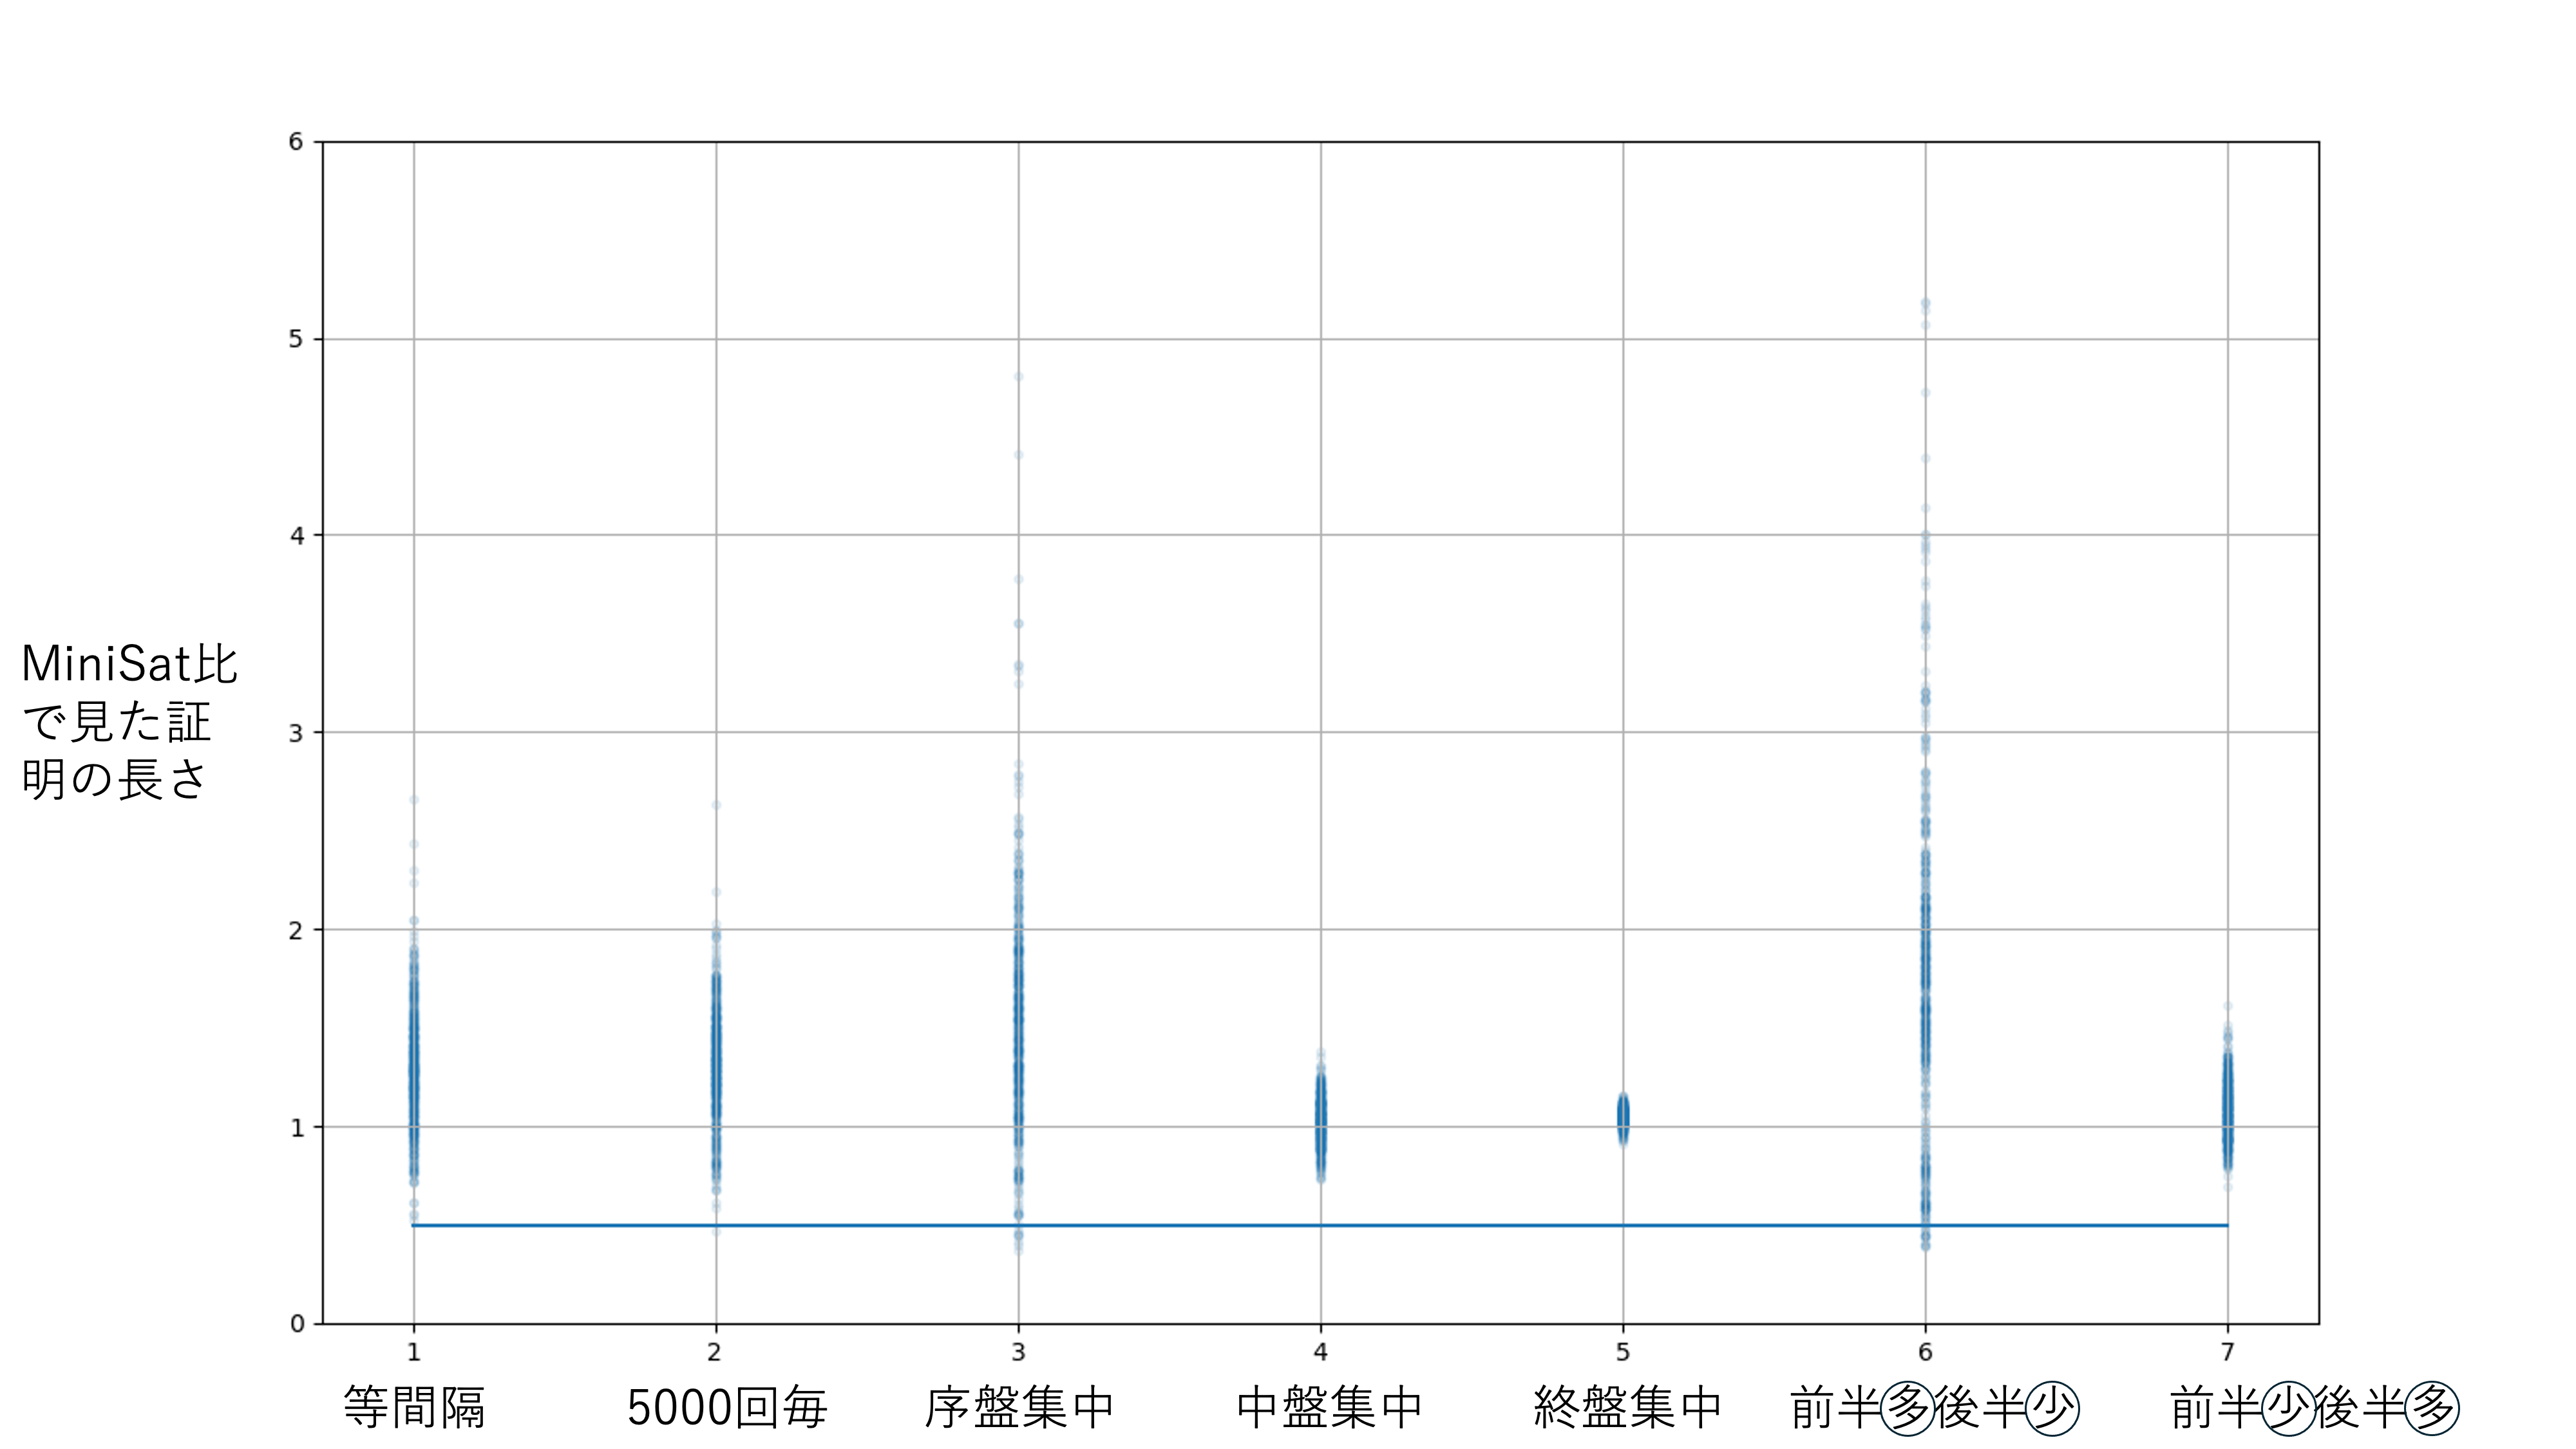
\includegraphics[width=10cm]{figures/Experiment0/1.png}
    \caption{タイミングずらしつつ8回介入(あとでちゃんとした画像に)}
\end{figure}





\subsection{パラメータ調整}%5ページ



まず最初の実験として遺伝アルゴリズムのパラメータ調整を行う実験を行なった。
問題を1つ固定し、遺伝アルゴリズムがより効果的に作用するようにパラメータの調整をしている。
調整を行なったのは以下の4つで、実験によってそれぞれ
\begin{itemize}
    \item 初期集団を作成する際の各染色体の介入数はランダムに選択
    \item 集団のサイズを200
    \item 世代数は30世代
    \item 突然変異を行う際は元の介入の1割を追加・削除
\end{itemize}
といった調整がなされている。
問題はあまり時間がかからない数秒で解けるような問題
\footnote{MiniSatで1.7秒、drat-trimで2.9秒ほどかかる問題で、証明の長さが約25000、変数選択数が約40000回の問題}
を採用した。

% 通常の6000倍ぐらいの実行時間
% 遺伝アルゴリズムはパラメータ調整がが必要


\subsubsection{初期状態}
\begin{figure}[h]
    \centering
    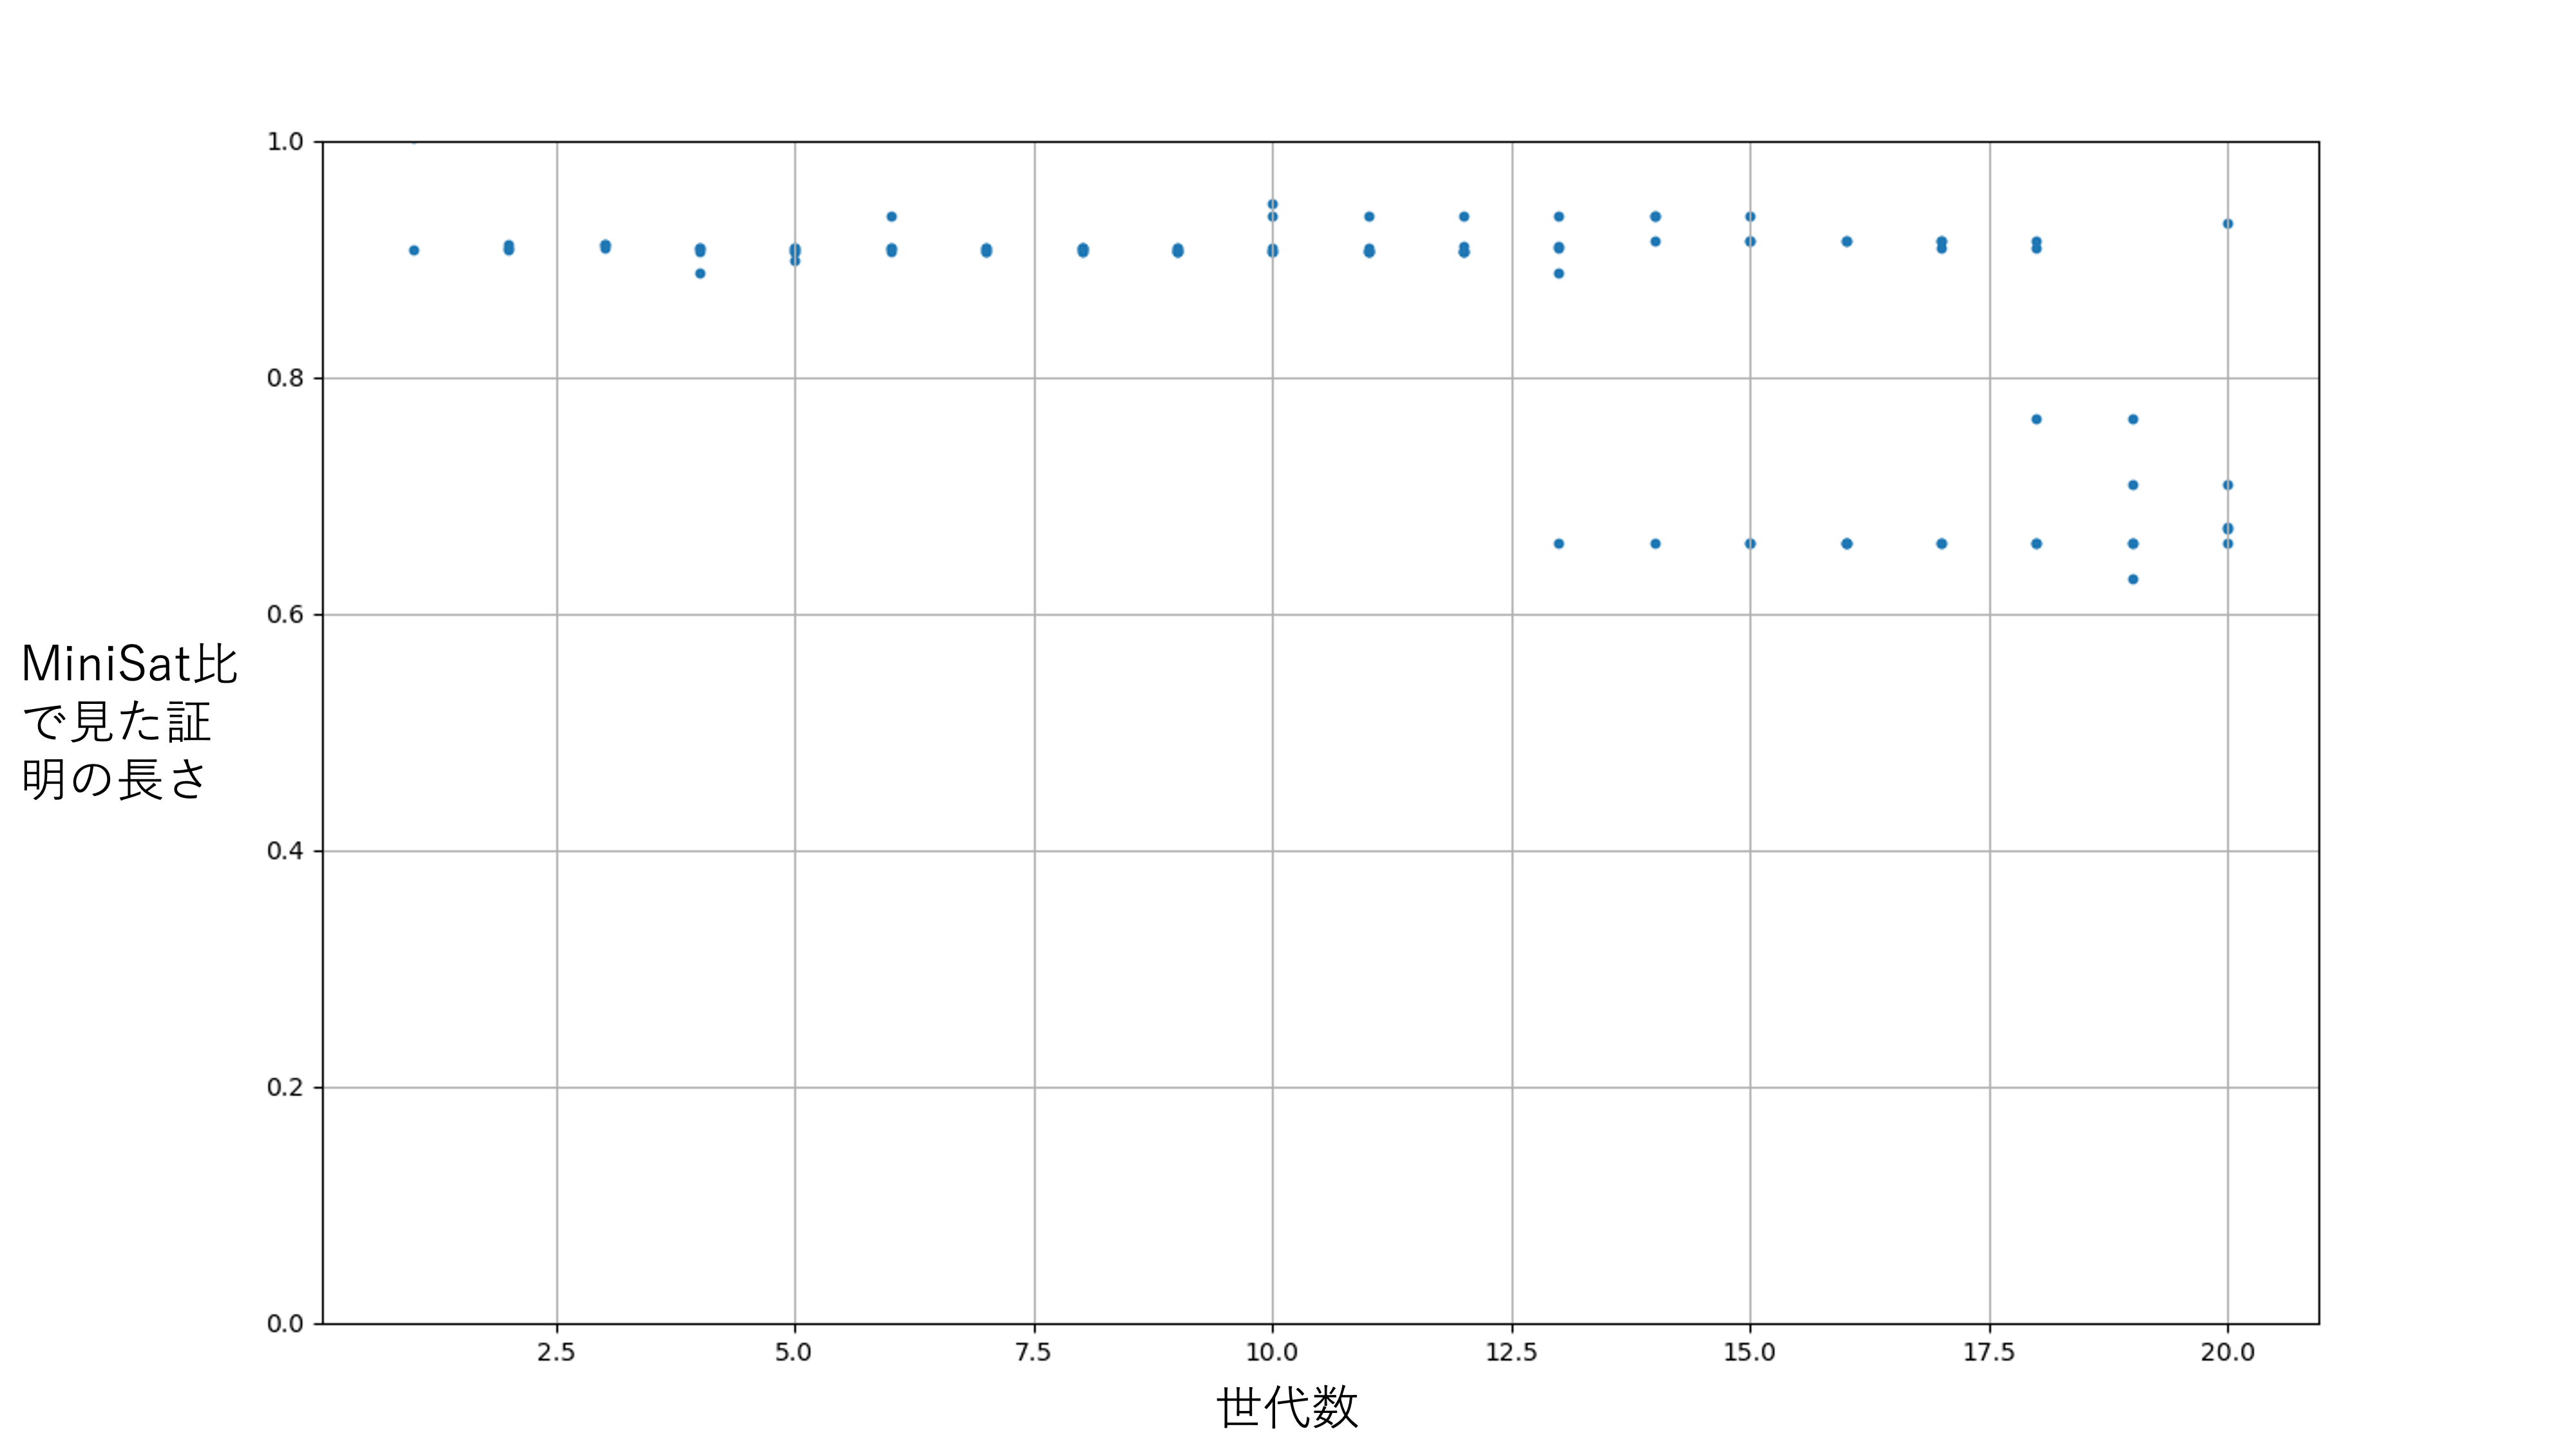
\includegraphics[width=10cm]{figures/Experiment1/1.png}
    \caption{初期パラメータにおける全染色体の証明長}
\end{figure}
最初に現在の遺伝アルゴリズムを実行しその効果を見た。
集団サイズは5で20世代まで作成、初期集団の各染色体の介入の回数は10回で固定し、
突然変異の際の介入の追加・削除数は1としてる。
結果を見ると13世代目で大きく良い個体が作成されているだけで、
それ以外の世代では大きく良い個体が作成されているような箇所はない。
また各染色体に距離があり、集団のサイズが少なく多様性がないように感じられる。
そのため次に集団の多様性を上げるような調整を行なった。
なお、ここでの一番短い証明はもとの証明の60\%ほどの証明であった。



\subsubsection{集団サイズと世代数を増加}
\begin{figure}[h]
    \centering
    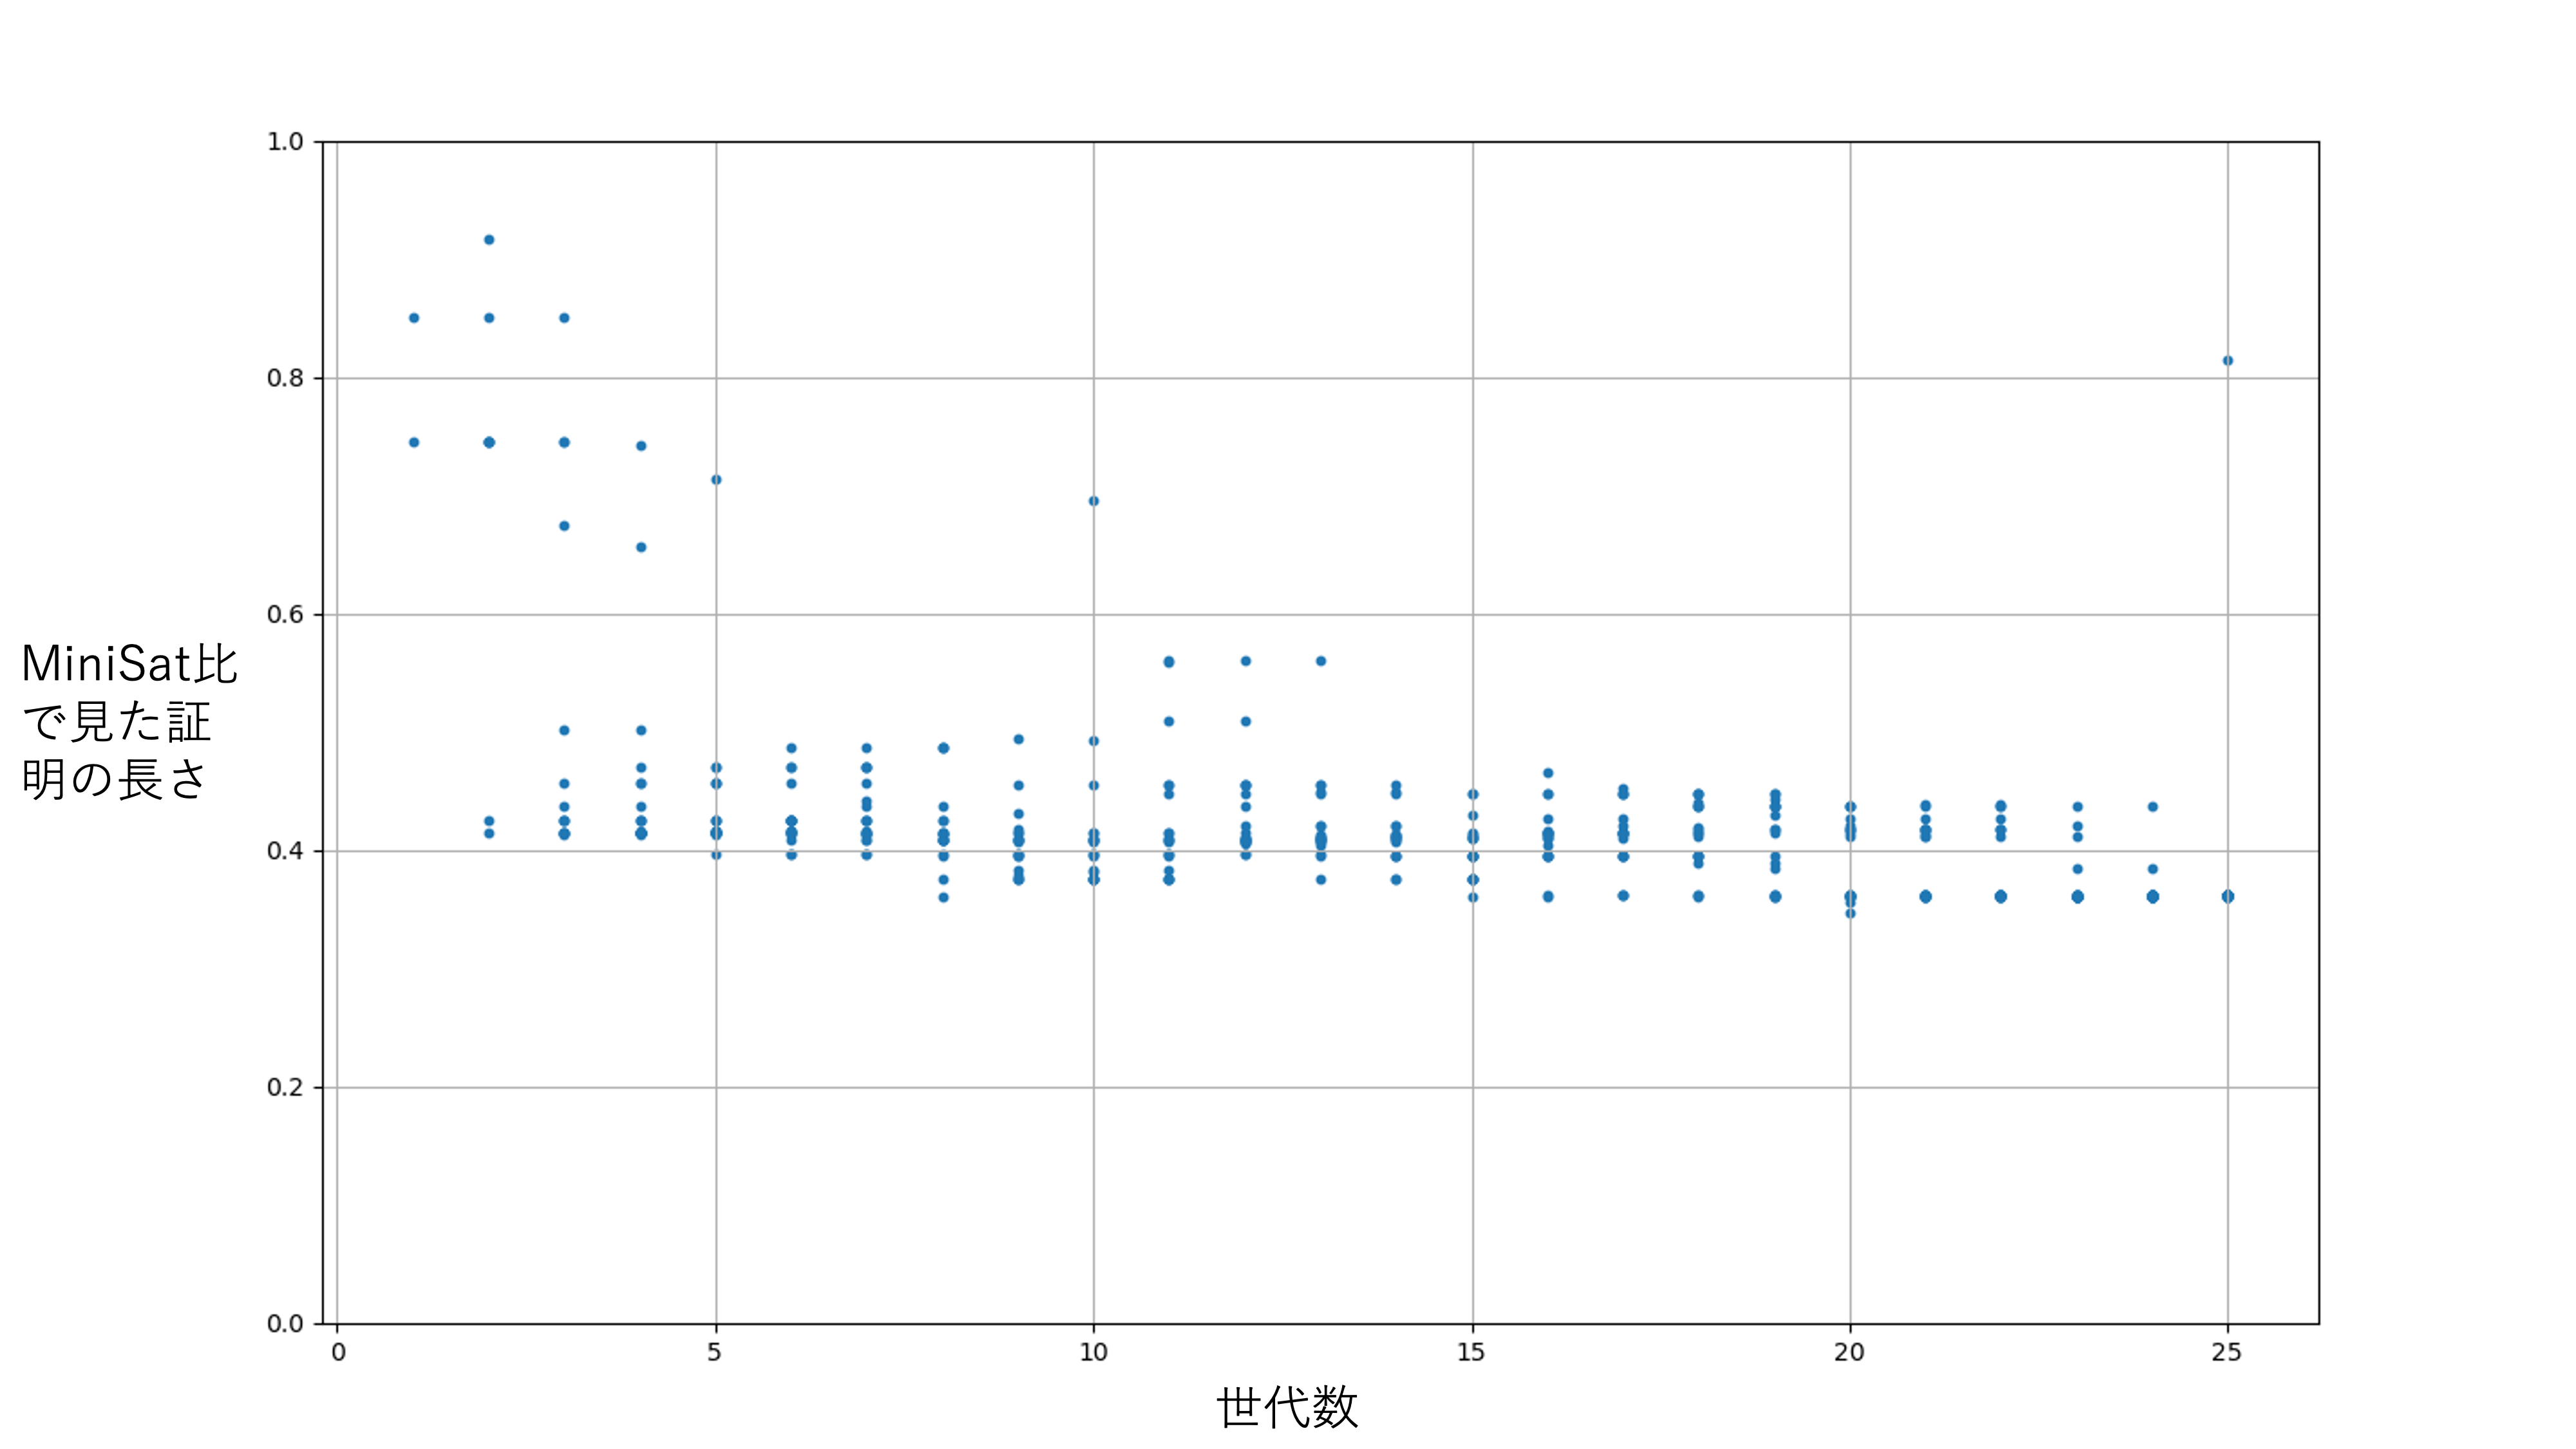
\includegraphics[width=10cm]{figures/Experiment1/2.png}
    \caption{集団サイズと世代を増加}
\end{figure}
次の実験では集団のサイズと世代数を増やす調整を行なった。
ここでは集団のサイズを20、世代数を25にして増やした上で遺伝アルゴリズムを実行した。
この変更によって集団の多様性が増え、より短い証明が作成されることを期待している。
結果として初期の結果よりも短い証明を作成することができた。
2世代目で良い個体を作ることができているが、
5世代目以降ではほとんどの個体が50\%弱のあたりに集まる形になっており、すぐに収束してしまっている。



\subsubsection{介入の回数をランダムに}

 ・20 * 25

 ・初期介入回数ランダム

\begin{figure}[h]
    \centering
    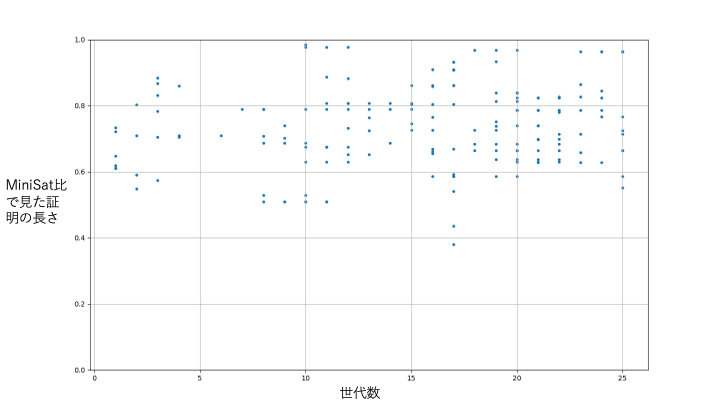
\includegraphics[width=10cm]{figures/Experiment1/3.png}
    \caption{初期の介入回数をランダムに}
\end{figure}

 ・多様性が増えた

 ・どの介入もなんか収束してそう

\begin{figure}[h]
    \centering
    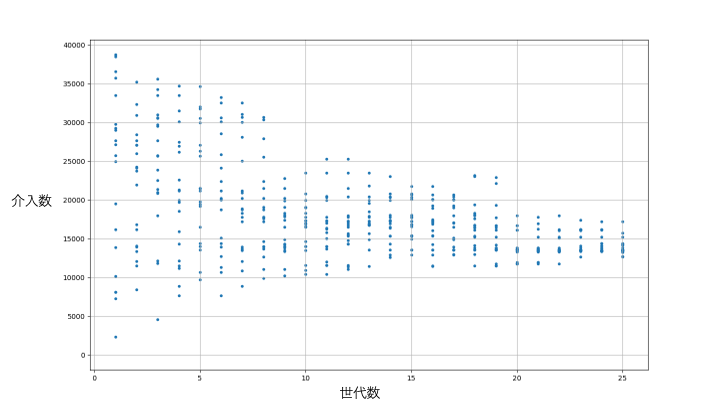
\includegraphics[width=10cm]{figures/Experiment1/3-1.png}
    \caption{介入回数の遷移}
\end{figure}

  ・初期の介入回数を10000以上20000以下に

\begin{figure}[h]
    \centering
    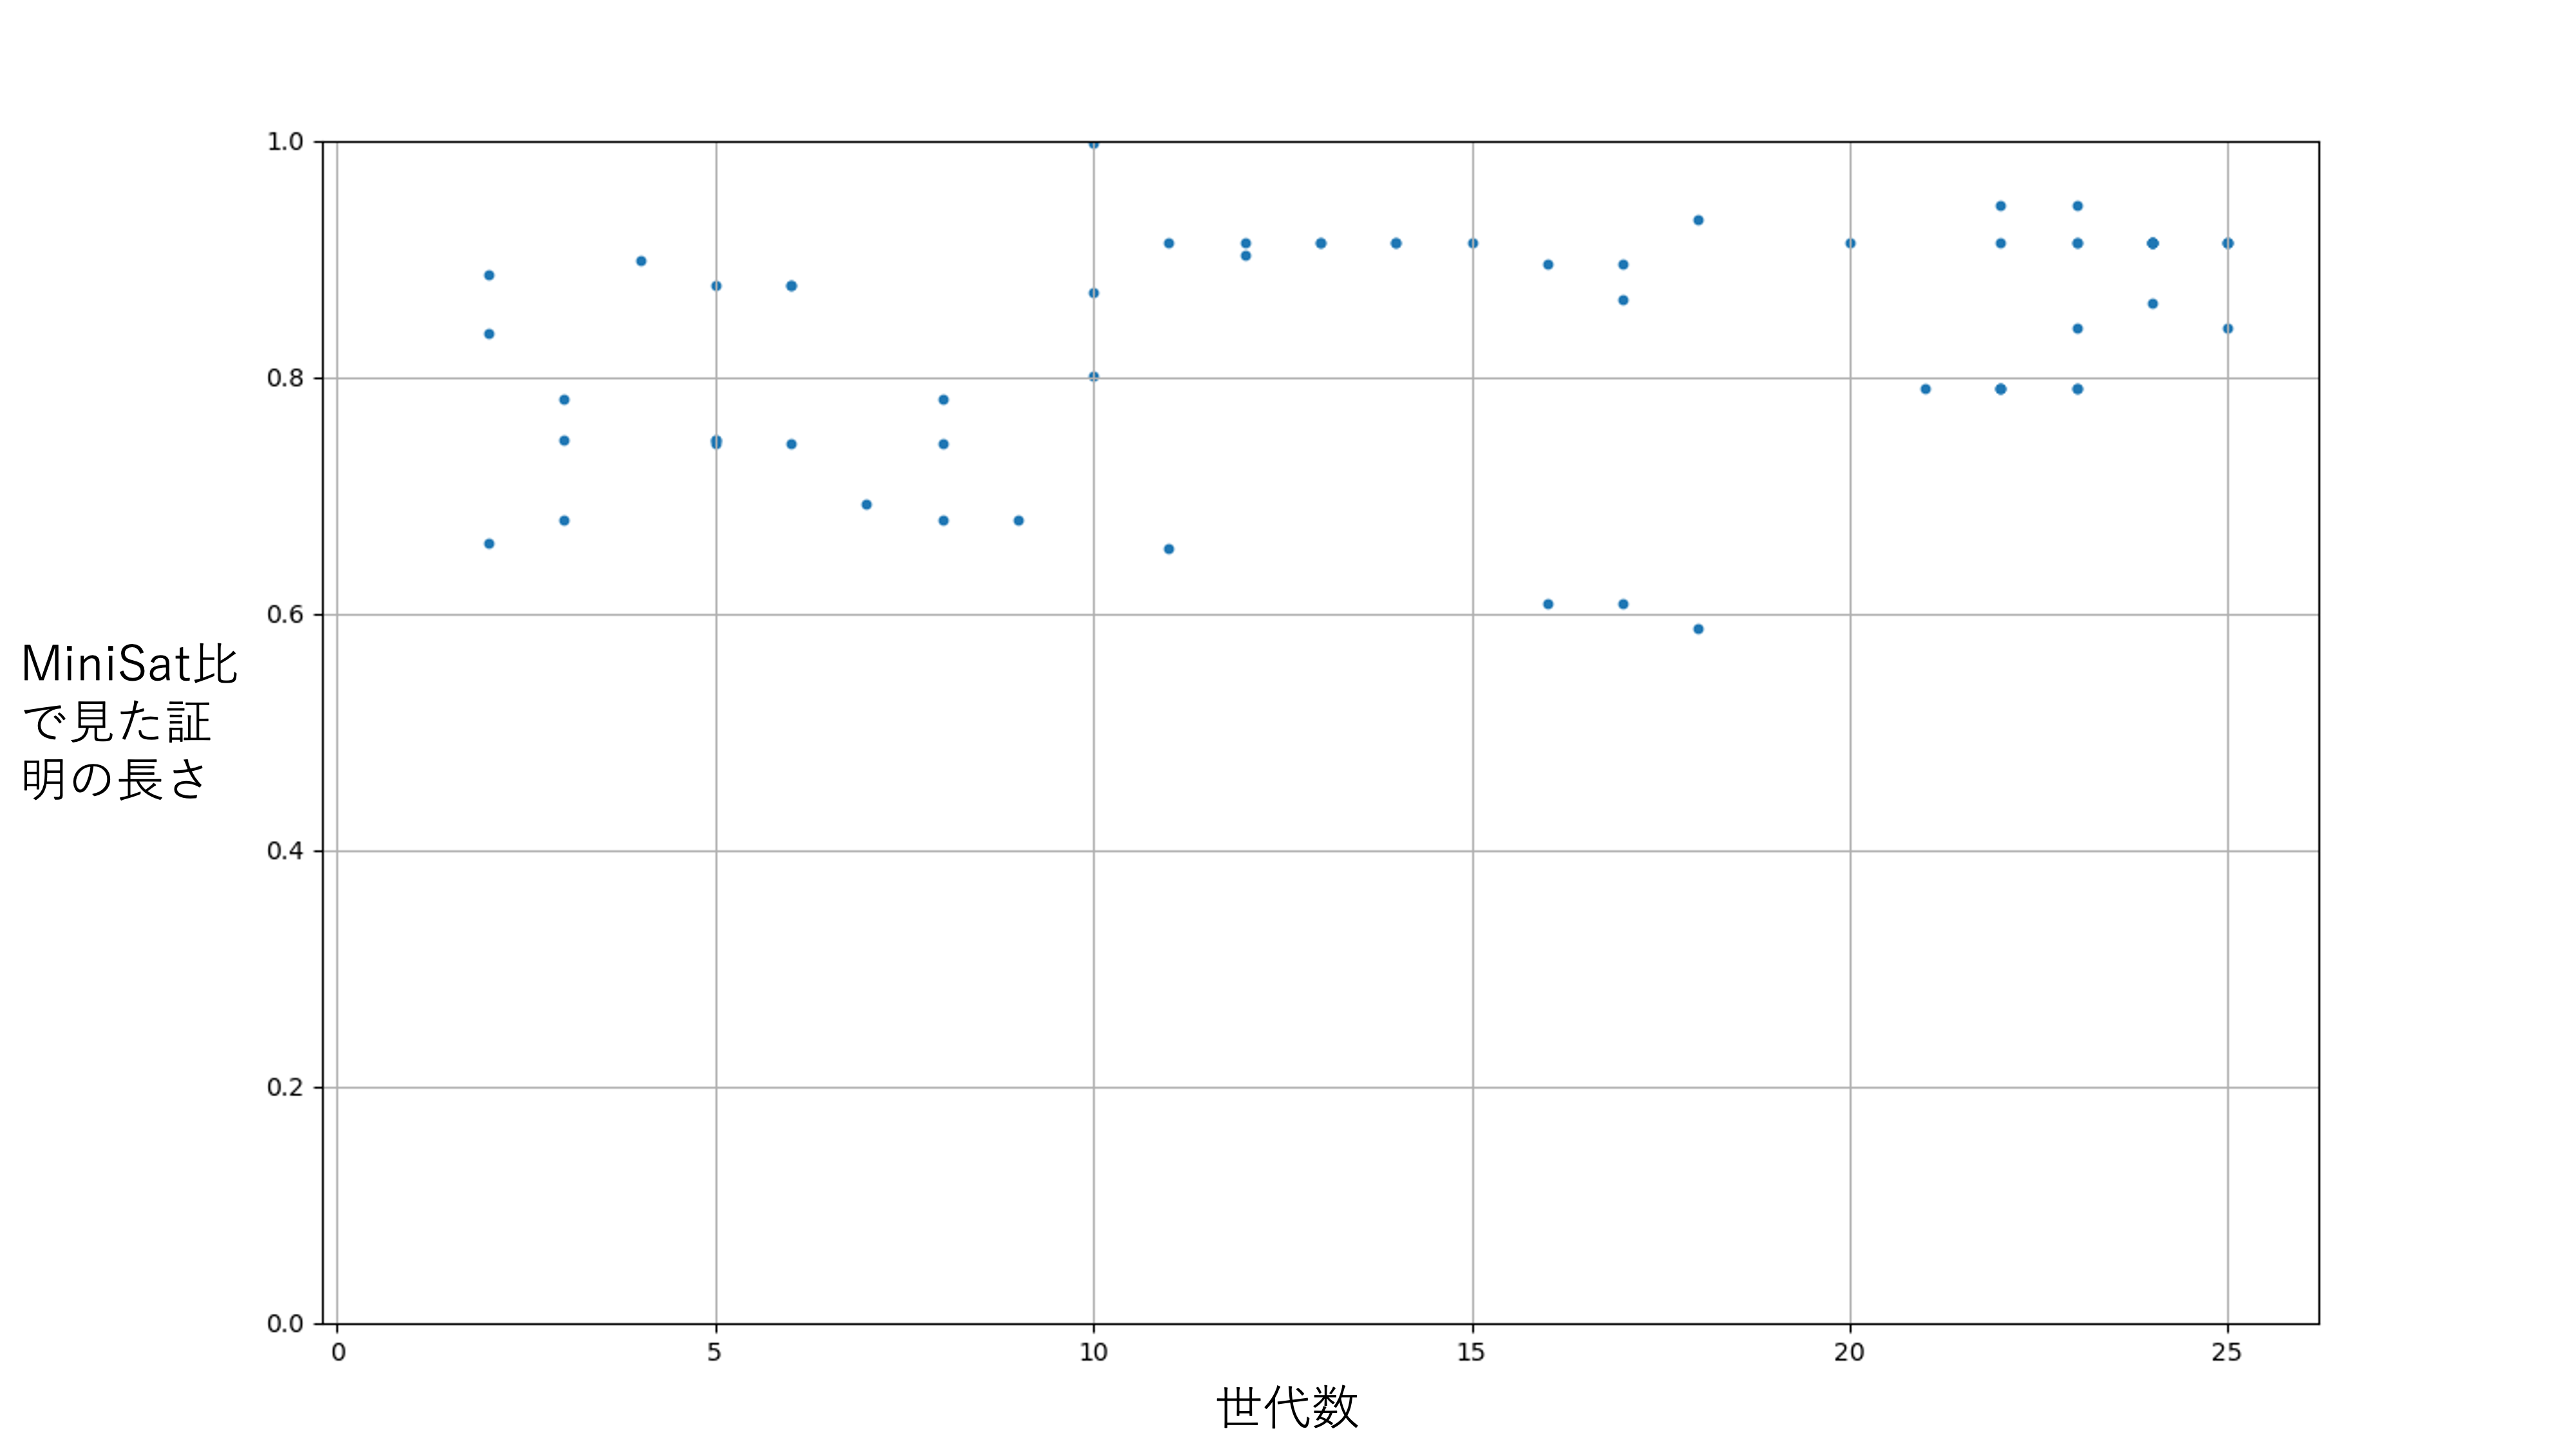
\includegraphics[width=10cm]{figures/Experiment1/3-2.png}
    \caption{介入回数を10000以上20000以下で始める}
\end{figure}

・介入をランダムにしてその状態での集団サイズと試行回数を調べた

4集団サイズと世代の変更

\begin{figure}[h]
    \centering
    \begin{minipage}{0.43\columnwidth}
        \centering
        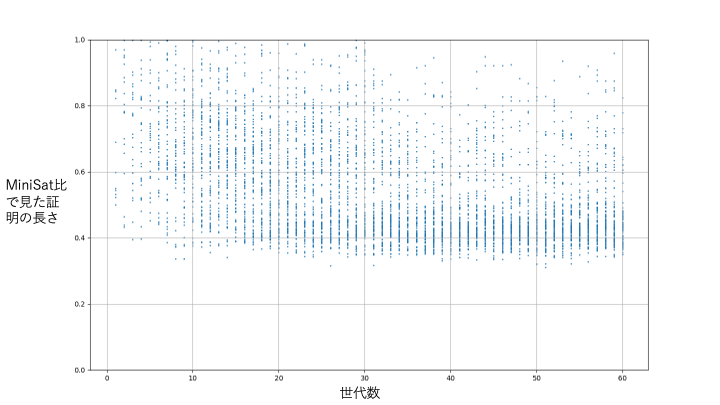
\includegraphics[width=\columnwidth]{figures/Experiment1/4-1.png}
        \caption{集団サイズ100、世代数60}
        \label{fig:サンプルA}
    \end{minipage}
    \hspace{5mm}
    \begin{minipage}{0.43\columnwidth}
        \centering
        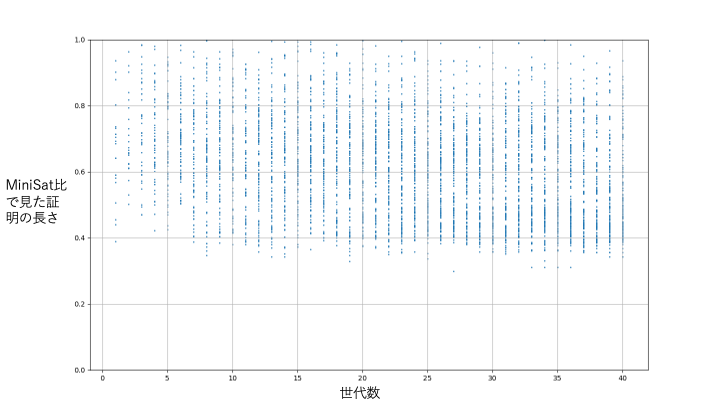
\includegraphics[width=\columnwidth]{figures/Experiment1/4-2.png}
        \caption{集団サイズ150、世代数40}
        \label{fig:サンプルB}
    \end{minipage}
  
    \vspace{3mm}
    
    \begin{minipage}{0.43\columnwidth}
        \centering
        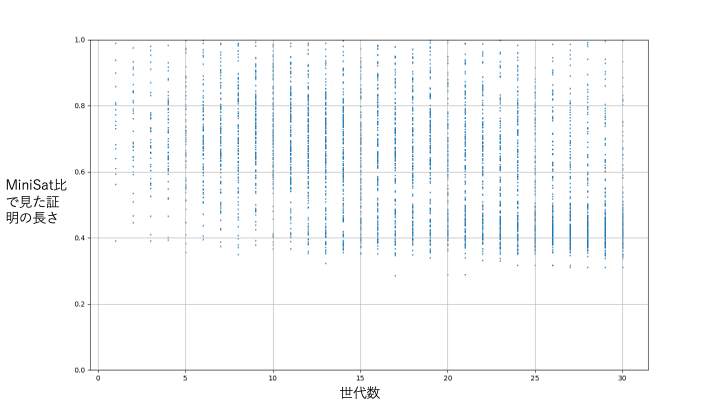
\includegraphics[width=\columnwidth]{figures/Experiment1/4-3.png}
        \caption{集団サイズ200、世代数30}
        \label{fig:サンプルC}
    \end{minipage}
    \hspace{5mm}
    \begin{minipage}{0.43\columnwidth}
        \centering
        
\includegraphics[width=\columnwidth]{figures/white.png}
    \end{minipage}
    \caption*{評価回数を6000として集団サイズと世代を変更}
\end{figure}

% 横にランダムと初期状態のベスト置きたい
5突然変異の変更
\begin{figure}[h]
    \centering
    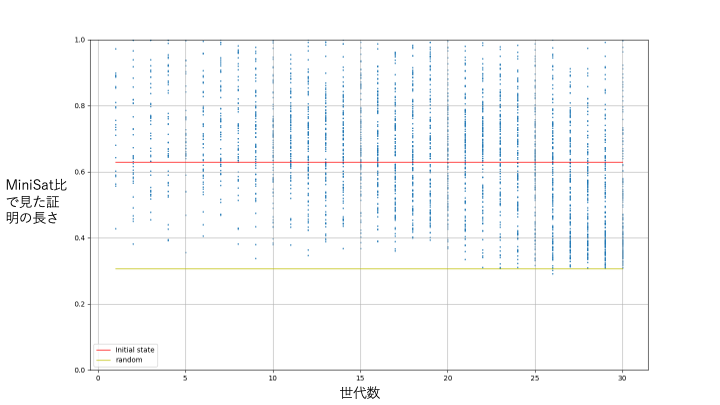
\includegraphics[width=10cm]{figures/Experiment1/5.png}
    \caption{突然変異の変更}
\end{figure}

6ランダムとの比較

7trim前の適応度の比較

 ・実行時間を短縮できないかという目的



\subsection{色々な問題に対して解く}%6ページ

・同じくらいの問題を解く

・長い問題を解く

・各問題のベストを見る

・空いている部分の問題を解く

・学習が続いている問題をを解く



\subsection{kissatとの比較}%4ページ

・kissatとの比較



\subsection{今後のために少し調べたこと}

・適応度を2乗に










\section{結果}
今回作成した遺伝アルゴリズムとMiniSatを使用することによって、
もとのMiniSatよりも短い証明を作成することができた。
どの問題に対しても短い証明を作成することができたがその短さには幅があり、
短いものだともとの10\%ほどの長さの証明作成できているが、
長いものだともとの85\%ほどの長さの証明を作成していた。
また、この作成した証明と最先端ソルバの1つであるKissatが作る証明を比較したところ、
ほとんどの問題においてKissatよりも短い証明を作成できなかったという結果を得た。
また、勝てているような証明についてもほとんどがKissatの証明と差があまりないという結果であった。
このようにKissatに大幅に勝てたような証明を作れなかった原因として考えられる可能性は3つあり、
変数選択以外の部分でMiniSatとKissatに大きな差がある可能性、
今回作成した遺伝アルゴリズムが適切に実装できていないもしくは適切な調整を行なったところで勝てないぐらいそもそも遺伝アルゴリズムに効果がない可能性。
Kissatが作成する証明がすでにほぼ最適解をたたきだしておりどう頑張ってもこれより大幅に短い証明を作れない可能性が考えられる。










\section{今後の課題}

今後の課題としては前述した3つの可能性の中でどの可能性がもっともあり得るのかを調べることが1つの課題として挙げられる。

1つ目の可能性として変数選択への介入ではMiniSatがKissatに勝てない可能性がある。
MiniSatとKissatの大きな違いとして証明の作り方に大きな違いがあるため。
証明の構造を調査することによってその可能性を確かめることができるかもしれない。
MiniSatは前処理の中で新しく節を作成する操作をおこなっているが
この操作をKissatは探索の中でも新しく節を作成している。
そのため、この節の作成によってMiniSatよりも短い証明を作成している可能性はある。
DRATの検証の部分で2種類の検証を行なっていることを述べたが、
Kissatが探索中で新しく作成するような節と学習節として作成している節の検証は
別の検証をおこなっている。
そのため、MiniSatとKissatの証明において各節がどの検証を使用しているかを確認することで
KissatにおいてMiniSatが前処理で作成しているような節がどれだけ使用されているかを確認することができる。

2つ目の可能性として遺伝アルゴリズムに効果がない、適切に実装できていない可能性がある。
これについては遺伝アルゴリズムを変更してその場合に効果があるかどうかを確かめることが考えられる。
遺伝アルゴリズムには様々なパラメータがあるがまずその1つとして染色体の表現方法がある。
今回はタイミングを最初から数えた変数選択数として表現しているが、
他の表現方法としてこのタイミングを前の介入タイミングから数えて何回目の変数選択数で表現する方法などが考えられる。

またオペレータとして交叉と突然変異を使用したがこの方法についても別の方法が考えられる。

交叉においては今回1点交叉を採用しておりタイミングを1つ決めてそれ以降で交換しているが、
それぞれの親に対して同じ交換位置である必要はなく別の交叉位置で交換する方法も考えられる。
交叉位置の候補としてはまず1つにランダムに決める方法があり、他にも変数の重みが似ているような介入以降で交換する方法もある。
後者の交叉位置の設定は、2つの移動経路の交叉を考える際に片方のある地点と近い地点をもう片方の移動経路から探し出し、
その地点以降で交換する方法と似ている。
また1点交叉によってあるタイミング以降を交換するのではなく、
あるタイミングから別のタイミングまでの一部分を交換する2点交叉なども考えられる。

突然変異については介入を削除・追加以外にもいくつかの方法を考える考えることができる。
例えばタイミングを少し前後にずらす方法がある。
タイミングを少しずらしその介入の直後に矛盾を引き起こした場合、
新しい重みの計算や別の学習節を作るため別の探索になる可能性がある(もちろんその逆もあり得る)。
またタイミングではなくシード値のみを変える方法や介入の順序を変える方法もある。

他にも変数の重みをランダムで書き換えていたが別の書き換え方法なども検討することができる。
MiniSatは前処理の段階で矛盾が起きた場合の重みの計算とは別の重みの計算を行なっており、
この重みの書き換えを探索の途中で再度計算する方法も考えられる。

3つ目の可能性としてKissatの証明がほぼ最適解の可能性が考えられる。
もし仮に実際にKissatに手を加えることで証明を減らすことができた場合、
Kissatの証明は最適解ではなく改善の余地があることになる。
今回MiniSatに行なった介入や遺伝アルゴリズムをKissatに行なった時に、
短い証明を作れるかどうかはこの可能性を確かめるための実験の1つである。












\section{まとめ}

本研究では変数選択への介入と遺伝アルゴリズムを組み合わせて短い証明を作成した。
既存のソルバに対して累計変数選択数と書き換えの方法を指定することで別の探索を行い新しい証明を作成、
更に遺伝アルゴリズムを使用して短い証明を作れるような介入列の探索を行なった。
介入を行うソルバはMiniSatを使用した。

結果としてもとのMiniSatが作成する証明よりも短い証明を作成することができたが、
最先端のソルバーであるKissatが作成する証明より短い証明はほとんどできなかった。

この原因として考えられることして3つの可能性があり、
変数選択とは別の処理が証明の長さの差を生み出しておりMiniSatに対して適切な変数選択を行なったとしてもKissatに勝てない可能性、
遺伝アルゴリズムに効果がないためにKissatに勝てない可能性、
Kissatの証明がほぼ最適解であり近づくことはできてもKissatより大幅に短い証明を作れない可能性、
の3つの可能性が考えられる。

今後の実験としてはこの3つの可能性について検討するための実験が考えられる。
例えばKissatがほぼ最適解である可能性に対しては、
今回行なった変数選択への介入と遺伝アルゴリズムを実際にKissatに組み込んでみることなどがある。









% 参考文献
\bibliographystyle{jabbrv} %日本語の場合は jabbrv などとする
\bibliography{references}










\end{document}